\chapter{Run II Preparation}
\label{CHAPTER:RunIIPreparation}

\glsresetall % Resetting all acronyms

After the successful completion of the the first data taking period, the \gls{LHC} Run I, the accelerator and detectors went through a two year long technical shut-down which was designated the \gls{LS1}. During the period the accelerator completed a consolidation and improvement program to allow a ramp up of the beams energy up to the design value of $7\,\TeV$ per beam in proton-proton mode. At the same time the experiments also performed maintenance, repair and improvement programs. 

Data analysis continued during this period of no data taking using the datasets already available or the newly reconstructed parked data. After this final work over $8\,\TeV$ data was completed most \gls{CMS} physics analysis started their preparation for the \gls{LHC} Run II, where higher collision energies, even higher values of \gls{PU} and more recorded integrated luminosity are expected. Following this global effort the \gls{CMS} \gls{VBF} Higgs to invisible analysis also started its own preparation work. 

The first step is always the definition of a trigger condition for data taking. The effort made to create and study such an adequate set of trigger for the use of this analysis during run II is documented in section \ref{SECTION:RunIITriggerStudies}. Additionally, work was made to study and propose the creation of a dedicated \gls{QCD} \gls{MC} sample with signal like characteristics expanding on the one already created for Run I. This study can be found in section \ref{SECTION:RunIIQCDMonteCarloSamples}.

%%%%%%%%%%%%%%%%%%%%%%%%%%%%%%%%%%%%%%%%%%%%%%%%%%%%%%%%%%%%%%%%%%%%%%%%%%%%%%%%%%%%%%%
%%% SECTION
%%%%%%%%%%%%%%%%%%%%%%%%%%%%%%%%%%%%%%%%%%%%%%%%%%%%%%%%%%%%%%%%%%%%%%%%%%%%%%%%%%%%%%%
\section{Run II trigger studies}
\label{SECTION:RunIITriggerStudies}

The first step of any \gls{CMS} physics analysis is to define which trigger to use for data taking. The \gls{TSG} develops generic usage trigger conditions, know as trigger paths, which can be used by any analysis. Typically this conditions cover all possible single objects (single electron, single jets, etc), multiple objects (double electron, triple muon, etc), cross triggers, (single electron $+$ sigle muon, etc). In some cases, like for our analysis, it with better to define a custom condition to obtain maximum physics content. The following reasons drove the decision to create a set dedicated trigger paths.

\begin{itemize}
  \item Maximize signal collection efficiency by selecting our signal topology with reduced trigger cuts while compared with generic triggers;
  \item Use again a trigger condition with $MET_{\text{no muon}}$ instead of $MET$ to study \gls{EWK} Z irreducible background;
  \item Create a new dedicate pre-scaled trigger path with reduced thresholds with objective of reducing systematics;
\end{itemize}

For the proposal of our triggers it was decided to produce numbers for conservative and aggressive scenarios in terms of available \gls{HLT} bandwidth. For the signal trigger path rate $1.5\,\hertz$ and $5.0\,\hertz$ were considered. While for the systematics paths rate $0.1\,\hertz$ and $0.1\,\hertz$ were considered.

\subsection{Methodology}



\subsection{Signal path}


% 2a) lowest MET cut (with >3% efficiency)
% * 1.5Hz - L1T_ETM70 + HLT_DijetVBF60-60_DEta3.5_MJJ700 + pf_met=144 rate=1.5Hz signalEff=0.0303
% * 5.0Hz - L1T_ETM + HLT_DijetVBF100-40_DEta2.5_MJJ1100 + pf_met=122 rate=4.96 signalEff=0.0301 (this is the highest MJJ point I have maybe it can go higher)
% * 5.0Hz - L1T_ETM + HLT_DijetVBF60-60_DEta3.9_MJJ700 + pf_met=125 rate=4.91 signalEff=0.031
% 
% 2b. best efficiency for dijet pT>40 GeV (other cuts can vary)
% * 1.5Hz - L1T_ETM70 + HLT_DijetVBF40-40_DEta2.5_MJJ500 + pf_met=164 rate=1.08 signalEff=0.0476
% * 5.0Hz - L1T_ETM70 + HLT_DijetVBF40-40_DEta2.5_MJJ500 + pf_met=152 rate=4.83   Hz signalEff=0.0546
% 
% 4a) run plot making on 3. and search for working points with maximum additional efficiency
% Sadly value are a bit low:
% * 1.5Hz - L1T_ETM70 + HLT_DijetVBF60-40_DEta3.7_MJJ500 + pf_met=152 rate=1.46 signalEff(NOT HLT_PFMET170)=0.009 (asymmetric)
% * 1.5Hz - L1T_ETM70 + HLT_DijetVBF40-40_DEta3.5_MJJ600 + pf_met=152 rate=1.42 signalEff(NOT HLT_PFMET170)=0.0087 (symmetric)
% * 5.0Hz - L1T_ETM70 + HLT_DijetVBF60-40_DEta3.7_MJJ500 + pf_met=140 rate=4.36 signalEff(NOT HLT_PFMET170)=0.0155 (asymmetric)
% * 5.0Hz - L1T_ETM70 + HLT_DijetVBF40-40_DEta3.5_MJJ600 + pf_met=140 rate=4.21 signalEff(NOT HLT_PFMET170)=0.0149 (symmetric)
% 
% So with 5.0Hz we go for 9.4% from HLT_PFMET170 to 10.9% so an improvement of about 16%.

\subsection{Systematics path}

% From our discussion yesterday, I was asked to look at the path with no L1 seeded (HLT_PFMET_PFVBF_Unseeded_v1) for control trigger, so I only have results without L1 seeded for now (see below).
% 
% Here are the unprescaled rates from several (lower) PFMET thresholds 
% 
% HLT_DijetVBF35-35_DEta3.5_MJJ600_PFMET60
% unprescaled rate = 12553.82 Hz
% HLT_DijetVBF35-35_DEta3.5_MJJ600_PFMET70
% unprescaled rate = 8139.73 Hz
% HLT_DijetVBF35-35_DEta3.5_MJJ600_PFMET80
% unprescaled rate = 4831.11 Hz
% HLT_DijetVBF35-35_DEta3.5_MJJ600_PFMET90 
% unprescaled rate = 2675.93 Hz 
% HLT_DijetVBF35-35_DEta3.5_MJJ600_PFMET100 
% unprescaled rate = 1394.83 Hz 
% 
% HLT_DijetVBF40-40_DEta3.5_MJJ500_PFMET60
% unprescaled rate = 9001.48 Hz
% HLT_DijetVBF40-40_DEta3.5_MJJ500_PFMET70
% unprescaled rate = 5873.20 Hz
% HLT_DijetVBF40-40_DEta3.5_MJJ500_PFMET80
% unprescaled rate = 3495.69 Hz
% HLT_DijetVBF40-40_DEta3.5_MJJ500_PFMET90 
% unprescaled rate = 1949.82 Hz 
% HLT_DijetVBF40-40_DEta3.5_MJJ500_PFMET100 
% unprescaled rate = 1033.37 Hz 
% 
% HLT_DijetVBF40-40_DEta3.5_MJJ600_PFMET60
% unprescaled rate = 6905.91 Hz
% HLT_DijetVBF40-40_DEta3.5_MJJ600_PFMET70
% unprescaled rate = 4525.34 Hz
% HLT_DijetVBF40-40_DEta3.5_MJJ600_PFMET80
% unprescaled rate = 2690.04 Hz <=========================
% HLT_DijetVBF40-40_DEta3.5_MJJ600_PFMET90 
% unprescaled rate = 1504.46 Hz 
% HLT_DijetVBF40-40_DEta3.5_MJJ600_PFMET100 
% unprescaled rate = 795.24 Hz 
% 
% If we aimed for 0.5 Hz, we need prescale N ~5000 from path you suggest.
% 
% You can find rate plots of these working points in attachment. 

%%%%%%%%%%%%%%%%%%%%%%%%%%%%%%%%%%%%%%%%%%%%%%%%%%%%%%%%%%%%%%%%%%%%%%%%%%%%

% See below with L1_ETM70 seeded and attached plot for HLT_DijetVBF40-40_DEta3.5_MJJ600_PFMET. 
% 
% Yes. I got your points but to include other L1 seeds (not L1_ETM70), as you said, I need to modified Joao’s code and I haven’t figured out how to do this yet (it’s in my next to do list), so we decided to look at the path without L1 seeded first. And I agree that producing ntuples which contain L1/HLT jets and MET would make our life easier :) I will do that.
% 
% Cheers,
% Chayanit
% 
% HLT_DijetVBF35-35_DEta3.5_MJJ600_PFMET60 
% unprescaled rate = 152.28 Hz
% HLT_DijetVBF35-35_DEta3.5_MJJ600_PFMET70
% unprescaled rate = 134.91 Hz
% HLT_DijetVBF35-35_DEta3.5_MJJ600_PFMET80
% unprescaled rate = 112.70 Hz
% HLT_DijetVBF35-35_DEta3.5_MJJ600_PFMET90 
% unprescaled rate = 86.90 Hz 
% HLT_DijetVBF35-35_DEta3.5_MJJ600_PFMET100 
% unprescaled rate = 62.25 Hz 
% 
% HLT_DijetVBF40-40_DEta3.5_MJJ500_PFMET60
% unprescaled rate = 139.66 Hz
% HLT_DijetVBF40-40_DEta3.5_MJJ500_PFMET70
% unprescaled rate = 123.25 Hz
% HLT_DijetVBF40-40_DEta3.5_MJJ500_PFMET80
% unprescaled rate = 101.64 Hz
% HLT_DijetVBF40-40_DEta3.5_MJJ500_PFMET90 
% unprescaled rate = 76.71 Hz 
% HLT_DijetVBF40-40_DEta3.5_MJJ500_PFMET100 
% unprescaled rate = 53.77 Hz 
% 
% HLT_DijetVBF40-40_DEta3.5_MJJ600_PFMET60
% unprescaled rate = 117.72 Hz
% HLT_DijetVBF40-40_DEta3.5_MJJ600_PFMET70
% unprescaled rate = 103.05 Hz
% HLT_DijetVBF40-40_DEta3.5_MJJ600_PFMET80
% unprescaled rate = 84.18 Hz
% HLT_DijetVBF40-40_DEta3.5_MJJ600_PFMET90 
% unprescaled rate = 62.24 Hz 
% HLT_DijetVBF40-40_DEta3.5_MJJ600_PFMET100 
% unprescaled rate = 44.08 Hz 

%%%%%%%%%%%%%%%%%%%%%%%%%%%%%%%%%%%%%%%%%%%%%%%%%%%%%%%%%%%%%%%%%%%%%%%%%%%%

% I just got the rates from L1_ETM50 (requiring L1 MET > 50) with unseeded PF HLT.
% 
% L1_ETM50 + HLT_DijetVBF40-40_DEta3.5_MJJ600_PFMET80 : unprescaled rate = 505.75 Hz
% 
% For 0.5 Hz, we need HLT prescale = 1
% 
% For 0.1 Hz, we need HLT prescale = 5
% 
% And see unprescaled rate plot in attachment.
% 
% PS. I found something’s a bit odd when I checked the rates between these two : 
% L1 MET > 70 + HLT_DijetVBF40-40_DEta3.5_MJJ600_PFMET80 (from unseeded path) rate = 182.03 Hz
% L1ETM70_HLT_DijetVBF40-40_DEta3.5_MJJ600_PFMET80 (using seeded path) rate = 84.18 Hz
% 
% Why are the rates different? Do I miss anything here?

%%%%%%%%%%%%%%%%%%%%%%%%%%%%%%%%%%%%%%%%%%%%%%%%%%%%%%%%%%%%%%%%%%%%%%%%%%%%

% OK, numbers are out:
% 
% * 1.5Hz - L1T_ETM70 + HLT_DijetVBF100-40_DEta3.7_MJJ500 + pf_met=150 rate=1.45Hz signalEff(NOT HLT_PFMET170)=0.008 (best eff asymmetric, different working point) 
% * 1.5Hz - L1T_ETM70 + HLT_DijetVBF40-40_DEta3.7_MJJ600 + pf_met=154 rate=1.46Hz signalEff(NOT HLT_PFMET170)=0.0075 (best eff symmetric, slight increase in thresholds) 
% * 1.5Hz - L1T_ETM70 + HLT_DijetVBF60-60_DEta3.7_MJJ1100 + pf_met=129 rate=1.44Hz signalEff(NOT HLT_PFMET170)=0.0062 (lowest met, now showed before)
% 
% * 5Hz - L1T_ETM70 + HLT_DijetVBF60-40_DEta3.7_MJJ500 + pf_met=140 rate=4.84Hz signalEff(NOT HLT_PFMET170)=0.0155 (best eff asymmetric, same WP with same sigEff and MET but rate increased)
% * 5Hz - L1T_ETM70 + HLT_DijetVBF40-40_DEta3.5_MJJ600 + pf_met=140 rate=4.68 signalEff(NOT HLT_PFMET170)=0.0149 (best eff symmetric, same WP with same sigEff and MET but rate increased)
% * 5Hz - L1T_ETM70 + HLT_DijetVBF60-40_DEta3.5_MJJ600 + pf_met=140 rate=4.48Hz signalEff(NOT HLT_PFMET170)=0.0148 (your request WP, same WP with same sigEff and MET but rate increased)
% * 5Hz - L1T_ETM70 + HLT_DijetVBF60-60_DEta4.1_MJJ800 + pf_met=119 rate=4.99Hz signalEff(NOT HLT_PFMET170)=0.0104 (lowest met, now showed before)
% 
% Code for additional L1T rate has run and first results will be computed as soon as I arrive to IC.
% 
% P.S.: I include the plot for your request WP which now shows no kink on rates.


%%%%%%%%%%%%%%%%%%%%%%%%%%%%%%%%%%%%%%%%%%%%%%%%%%%%%%%%%%%%%%%%%%%%%%%%%%%%%%%

% General points:
% * Control plots are unaffected. 
% * I think there may be a problem on my additional rate code. Its returning a total L1T rate of 130 kHz and some unexpected (higher than before) rates for the proposed dijet triggers. So I will do some debugging.
% 
% Will make some quick code to extract the individual efficiency of those proposed paths/
% 
% As for the default HLT:
% HLT_PFMET170_NoiseCleaned_v1 sigEff: 0.094 qcdRate: 4.515Hz

%%%%%%%%%%%%%%%%%%%%%%%%%%%%%%%%%%%%%%%%%%%%%%%%%%%%%%%%%%%%%%%%%%%%%%%%%%%%%%%

% => L1T_NoCuts/HLT_DijetVBF40-40_DEta3.5_MJJ600 + pf_met140=> Signal eff: 0.0515843 Total QCD Rate :4.67692
% => L1T_NoCuts/HLT_DijetVBF60-40_DEta3.5_MJJ600 + pf_met140=> Signal eff: 0.0512509 Total QCD Rate :4.48162


\section{Additional L1 trigger}

% Some new results for the "new L1T seed" DijetVBF30 + DEta3p5 + ETM50:
% 
% * 1.5Hz - HLT_DijetVBF100-40_DEta4.3_MJJ500 + pf_met=142 rate=1.49 signalEff(NOT HLT_PFMET170)=0.0101 (max efficiency)
% * 1.5Hz - HLT_DijetVBF60-60_DEta4.3_MJJ1100 + pf_met=132 rate=1.44 signalEff(NOT HLT_PFMET170)=0.0077 (lowest MET)
% 
% * 5.0Hz - HLT_DijetVBF60-40_DEta4.1_MJJ500 + pf_met=140 rate=4.77Hz signalEff(NOT HLT_PFMET170)=0.0171 (max efficiency)
% * 5.0Hz - HLT_DijetVBF60-60_DEta4.5_MJJ1000 + pf_met=122 rate=4.93Hz signalEff(NOT HLT_PFMET170)=0.0102 (lowest MET)
% 
% As expected with this seed we can get a bit more efficiency and go up to 11.1% an increase of 18.2% to just HLT_PFMET170
% 
% I will add tomorrow morning the study for the extra seed that had no L1T_ETM.

%%%%%%%%%%%%%%%%%%%%%%%%%%%%%%%%%%%%%%%%%%%%%%%%%%%%%%%%%%%%%%%%%%%%%%%%%%%%%%%%%%%%%%%
%%% SECTION
%%%%%%%%%%%%%%%%%%%%%%%%%%%%%%%%%%%%%%%%%%%%%%%%%%%%%%%%%%%%%%%%%%%%%%%%%%%%%%%%%%%%%%%
\section{Run II QCD Monte Carlo samples}
\label{SECTION:RunIIQCDMonteCarloSamples}

Simulating and reconstructing quantities of \gls{QCD} events comparable to the ones produced at the \gls{LHC} experiments is impractical. At every second of \gls{LHC} physics operation several millions of bunch crossings happen, each one able to create several simultaneous collisions. With the currently available hardware it takes in excess of one minute to fully simulate one of such bunch crossings. Further more, most of this events have very low energy collisions and are unlikely to be picked up by any physics analysis.  

This constraints lead to \gls{QCD} events being simulated in $p_\perp$ hats, where the first collision outgoing particles summed $p_\perp$ generated within a predefined rangee. Then several other collisions are added to the event as \gls{PU}. This additional collisions are generated without any constraints in $p_\perp$. 

This bin method allows the user to have \gls{QCD} hard scattering samples with increasing energies and study the influence of each one of them in their own analysis. As a practical example we do not need to look over millions of \gls{QCD} events to find high energy jets. We can just start from the higher \gls{QCD} $p_\perp$ hats add lower ones until the contributing to our selection is negligible. On the other hand, analysis like the \gls{CMS} \gls{VBF} Higgs to invisible analysis, search for event topologies with low energy jets and/or \gls{MET}. In this cases available inclusive \gls{QCD} samples will not have enough statistics to provide insight into this backgrounds behaviour. 

During the preparation of the Run I the \gls{VBF} Higgs to invisible analysis privately produced a set of \gls{QCD} samples with \gls{VBF} like jets and real \gls{MET}. This samples allowed to understand the mechanisms that create real \gls{MET} in \gls{QCD} and how those could be mitigated. 

In the preparation for Run II it was considered once again to be useful to have similar samples remade and possibly extended. It was identified that not only real \gls{MET} is significant but also fake \gls{MET} coming from detector miss-measurement. The \gls{QCD} background is currently the only background we do not have any \gls{MC} event sample. If such a sample could be produced it could allow the analysis to evolve to a shape based analysis or to use machine learning techniques, since we would have signal and all backgrounds simulations. 

\subsection{Monte Carlo sample simulation}

\glsreset{MC} methods are a class of computer algorithms that rely on random sampling to obtain numerical results. This type of methods is especially useful in problems with many coupled degrees of freedom where it is difficult to perform analytical calculations. In particle physics these methods are often used to simulate physics processes, their interaction with detectors and the obtained measurements.

To simulate one event on the \gls{CMS} experiment we first start by simulating the physics process itself. We can split this into two sub-processes: hard scattering and hadronization. There are many purpose developed software programs that will perform each one of this steps of even both. 

General purpose software like Pythia8 \cite{ARTICLE:Pythia6p4PhysicsAndManual,ARTICLE:Pythia8p1Introduction} or Herwig++ \cite{ARTICLE:HERWIGPhysicsAndManual} are able to do both hard scattering and hadronization. Typically these programs are restricted to 2 by 2 hard processes which are calculated at leading order. 

There are many other hard process only simulation programs 


\subsection{Final sample proposal}

%Status: Writing

Proposal to the Higgs sample generation contacts consists on the production of a MadGraph QCD sample with VBF characteristics and no missing transverse energy cut.

This sample is to be produced in two steps. The parton level simulation which is to be done with the MadGraph event generator. The base processes will be proton-proton to 2, 3, and 4 jets. Here a jet is defined as the hard process outgoing particle which can be a gluon or a quark (u, d, c, s or b). Only events with at least one outgoing di-parton where both parton have more than $30\,\GeV$ and at least $800\,\GeV$ are kept. 

The estimated cross section for this processes and selection is $1.11e+07 \pm 1.799e+04 \,\pico\barn$ and we request the production of $1.2 \time 10^{10}$ events. The corresponds to an equivalent luminosity of just over $1\,\femto\barn^{-1}$ of equivalent integrated luminosity.

The second step comprises the parton hadronization and event filtering. The objective is to further reduce the number of events without prejudice of physics usefulness of this sample. Hadronization is to be preformed with the \gls{MC} generator Pythia8 efficiency where the efficiency of the post hadronization event matching has been estimated of $9.0\% \pm 0.3\%$, leading to an sample cross section of $9.993e+05 \pm 3.127e+04 \pico\barn$. At this point we propose to separate the sample into two sub-samples according using a generator level filter. 

The first sample would be the result of running over all the events produced up to the hadronization step and select only the events with at least on generator level anti-$k_T^{\Delta T < 0.4}$ dijet where both jets have at least $\pt > 40\,\GeV$, $\Delta\eta > 3.0$, $m_{jj} > 1000\,\GeV$ and $\Delta\Phi<=2.15$. The estimated filter efficiency is $2.592e-02 \pm 2.541e-03$
which would lead to a sample since of approximately 26 million events and corresponding to an equivalent luminosity of over $1\,\femto\barn^{-1}$.

The second sample would be the result of running over only 10\% of the events available at the hadronization step. Here we reverse the $\delta\phi$ cut while keeping all that other cuts from the first sample. This filter has an efficiency of $2.592e-02 \pm 2.541e-03$  and would lead to sample of about 12 million events, corresponding to an equivalent luminosity of over $100\,\pico\barn$. If additional computing resources would become available this sample could be expanded up to 100\% of the base sample to a total of 120 million events and equivalent luminosity over $1\,\femto\barn^{-1}$.

%%%%%%%%%%%%%%%%%%%%%%%%%%%%%%%%%%%%%%%%%%%%%%%%%%%%%%%%%%%%%%%%%%%%%%%%%%%%%%%%%%%%%%%
%%% SUBSECTION
%%%%%%%%%%%%%%%%%%%%%%%%%%%%%%%%%%%%%%%%%%%%%%%%%%%%%%%%%%%%%%%%%%%%%%%%%%%%%%%%%%%%%%%
\subsection{Gridpack Validation}
\label{SUBSECTION:GridpackValidation}

% Total number of events: 17871
% 
% => Event counters:
% Jet Matched not lowest DeltaR : 1866
% Selected diparton has a match : 13218
% 
% pt>30 : 687 : 14 : 0.0203785 
% 
% pt>30 : 1467 : 49 : 0.0334015 

\begin{table}
\centering

\resizebox{1.0\textwidth}{!}{
\begin{tabular}{|c|c|c|c|c|c|}
\hline
                          & \multicolumn{3}{c|}{Events}      & \multicolumn{2}{c|}{Cross Section [pb]}                                       \\
\hline
Process                   & Tried  & Passed & accepted [\%]  & Before                                & After                                 \\
\hline\hline 
$p p \rightarrow j j$     &  30295 &   7252 & $23.9 \pm 0.2$ & $1.673e+06 \pm 8.616e+03$ & $4.005e+05 \pm 4.591e+03$ \\
$p p \rightarrow j j j$   &  64985 &   4776 & $ 7.3 \pm 0.1$ & $3.547e+06 \pm 1.826e+04$ & $2.607e+05 \pm 3.871e+03$ \\
$p p \rightarrow j j j j$ &  89720 &   5843 & $ 6.5 \pm 0.1$ & $4.939e+06 \pm 2.543e+04$ & $3.216e+05 \pm 4.393e+03$ \\
\hline\hline
Total                     & 185000 &  17871 & $ 9.7 \pm 0.1$ & $1.016e+07 \pm 3.247e+04$ & $9.828e+05 \pm 7.440e+03$ \\
\hline
\end{tabular}
}
\caption{TODO:}

\end{table}




% --------------------------------------------------------------------------------------------------------------------------------------------------------------------------                                                                                                    
% Overall cross-section summary                                                                                                                                                                                                                                                 
% --------------------------------------------------------------------------------------------------------------------------------------------------------------------------                                                                                                    
% Process         xsec_before [pb]                passed  nposw   nnegw   tried   nposw   nnegw   xsec_match [pb]                 accepted [%]     event_eff [%]                                                                                                                
% 0               1.673e+06 +/- 8.616e+03         7252    7252    0       30295   30295   0       4.005e+05 +/- 4.591e+03         23.9 +/- 0.2    23.9 +/- 0.2                                                                                                                  
% 1               3.547e+06 +/- 1.826e+04         4776    4776    0       64985   64985   0       2.607e+05 +/- 3.871e+03         7.3 +/- 0.1     7.3 +/- 0.1                                                                                                                   
% 2               4.939e+06 +/- 2.543e+04         5843    5843    0       89720   89720   0       3.216e+05 +/- 4.393e+03         6.5 +/- 0.1     6.5 +/- 0.1                                                                                                                   
% --------------------------------------------------------------------------------------------------------------------------------------------------------------------------                                                                                                    
% Total           1.016e+07 +/- 3.247e+04         17871   17871   0       185000  185000  0       9.828e+05 +/- 7.440e+03         9.7 +/- 0.1     9.7 +/- 0.1
% --------------------------------------------------------------------------------------------------------------------------------------------------------------------------
% Before matching: total cross section = 1.016e+07 +- 3.247e+04 pb
% After matching: total cross section = 9.828e+05 +- 7.440e+03 pb
% Filter efficiency (taking into account weights)= (17871) / (17871) = 1.000e+00 +- 0.000e+00
% Filter efficiency (event-level)= (17871) / (17871) = 1.000e+00 +- 0.000e+00
% After filter: final cross section = 9.828e+05 +- 7.440e+03 pb


\begin{table}[!htp]
\centering

\begin{tabular}{|c||c|c|c||c|}
\hline
            &          \multicolumn{4}{c|}{Process} \\
\hline
$n_{match}$ &      jj &    jjj  &    jjjj &   Total \\
\hline\hline 
          0 & 03.54\% &  0.29\% & 00.05\% & 01.53\% \\
          1 & 25.21\% &  4.23\% & 01.35\% & 11.80\% \\
          2 & 71.25\% & 27.55\% & 08.66\% & 39.11\% \\
          3 &         & 67.92\% & 36.16\% & 29.98\% \\
          4 &         &         & 53.77\% & 17.58\% \\
\hline
\end{tabular}
\caption{TODO:}

\end{table}

% => Parton to GenJet matching results:
% all partons entries 17871
% Matched #0 partons:  274 fraction: 0.0153321
% Matched #1 partons: 2109 fraction: 0.118012
% Matched #2 partons: 6989 fraction: 0.391081
% Matched #3 partons: 5357 fraction: 0.299759
% Matched #4 partons: 3142 fraction: 0.175816
% 
% jj partons entries 7252
% Matched #0 partons:  257 fraction: 0.0354385
% Matched #1 partons: 1828 fraction: 0.252068
% Matched #2 partons: 5167 fraction: 0.712493
% 
% jjj partons entries 4776
% Matched #0 partons:   14 fraction: 0.00293132
% Matched #1 partons:  202 fraction: 0.0422948
% Matched #2 partons: 1316 fraction: 0.275544
% Matched #3 partons: 3244 fraction: 0.679229
% 
% jjjj partons entries 5843
% Matched #0 partons:    3 fraction: 0.000513435
% Matched #1 partons:   79 fraction: 0.0135205
% Matched #2 partons:  506 fraction: 0.0865993
% Matched #3 partons: 2113 fraction: 0.361629
% Matched #4 partons: 3142 fraction: 0.537737


\begin{figure}[htp]%
\centering
\subfloat[][]{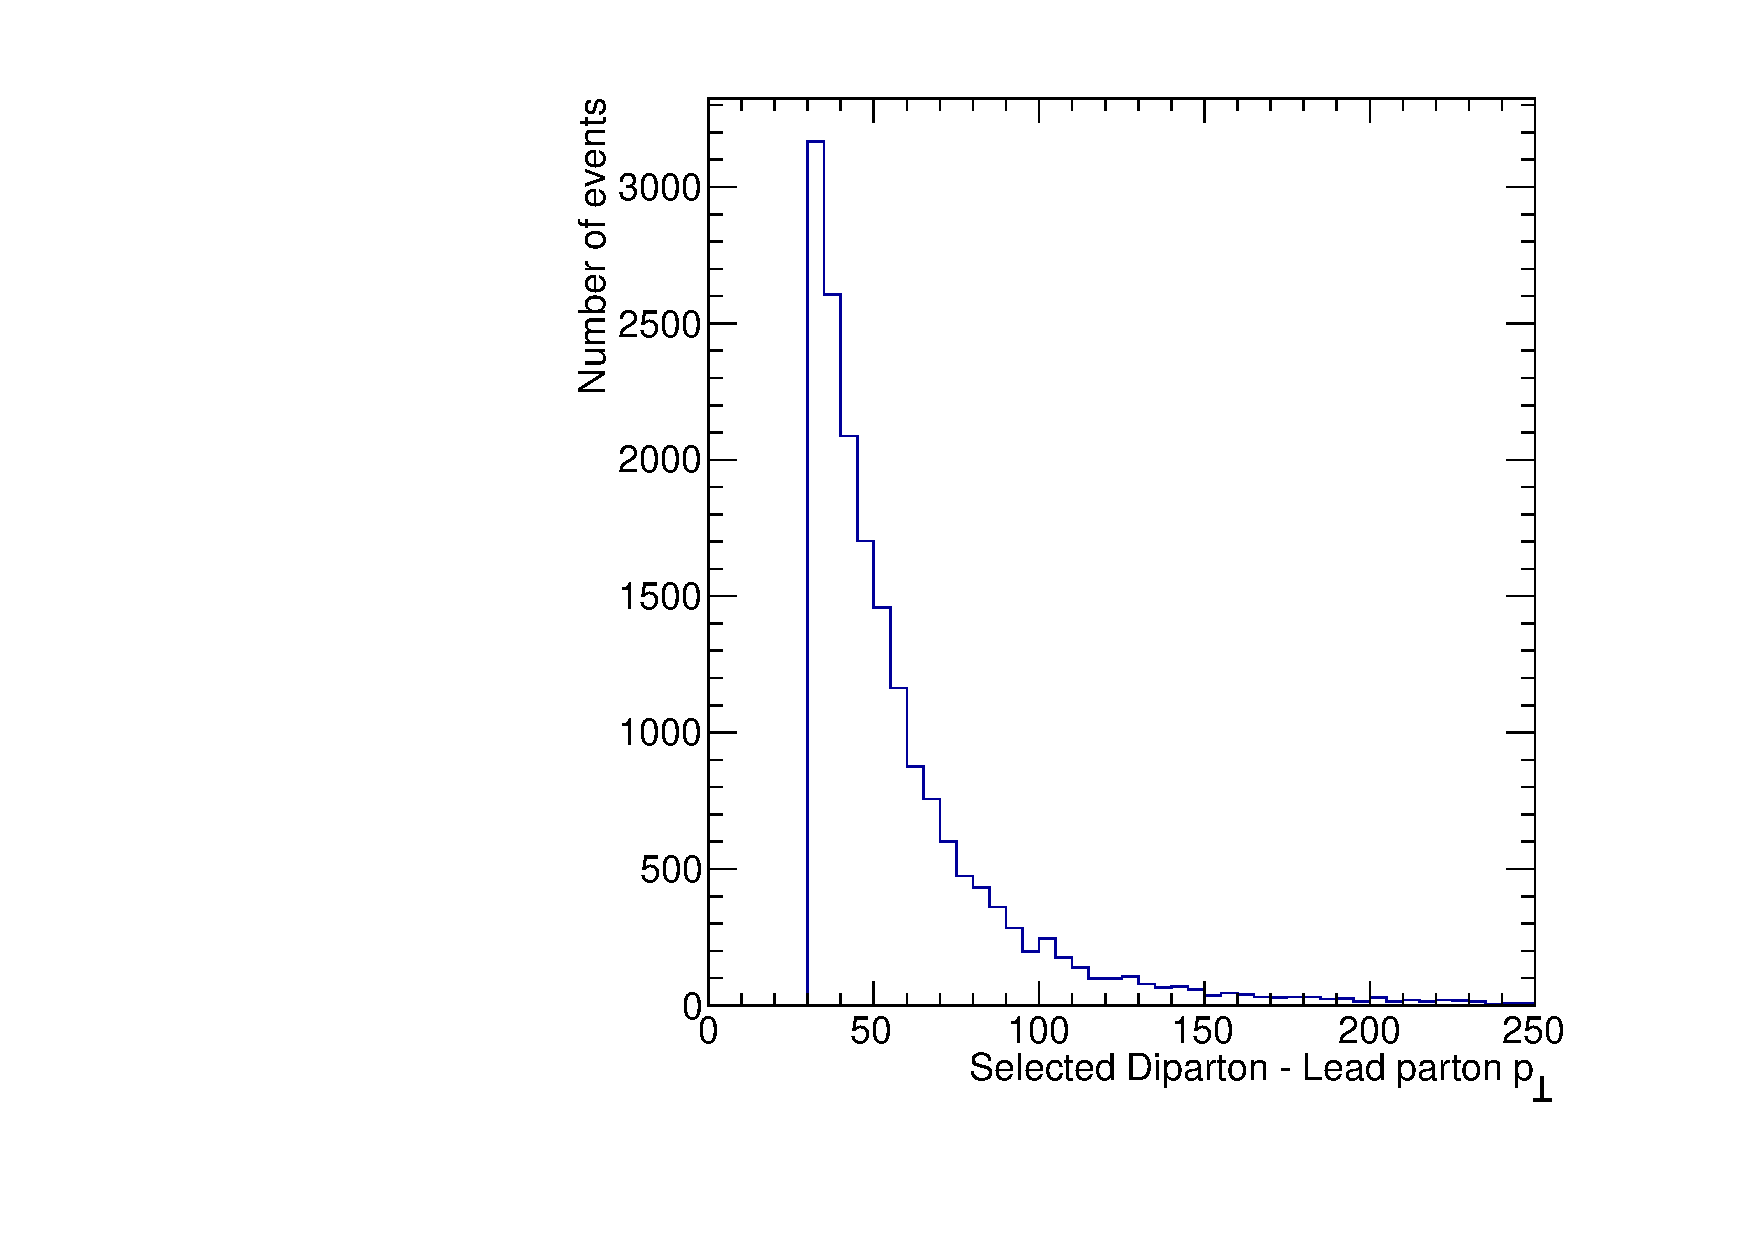
\includegraphics[width=0.45\linewidth]{Chapter07/QCDVBFSamples/Gridpack/Images/SelDiParton_Parton1_Pt.pdf}}\qquad
\subfloat[][]{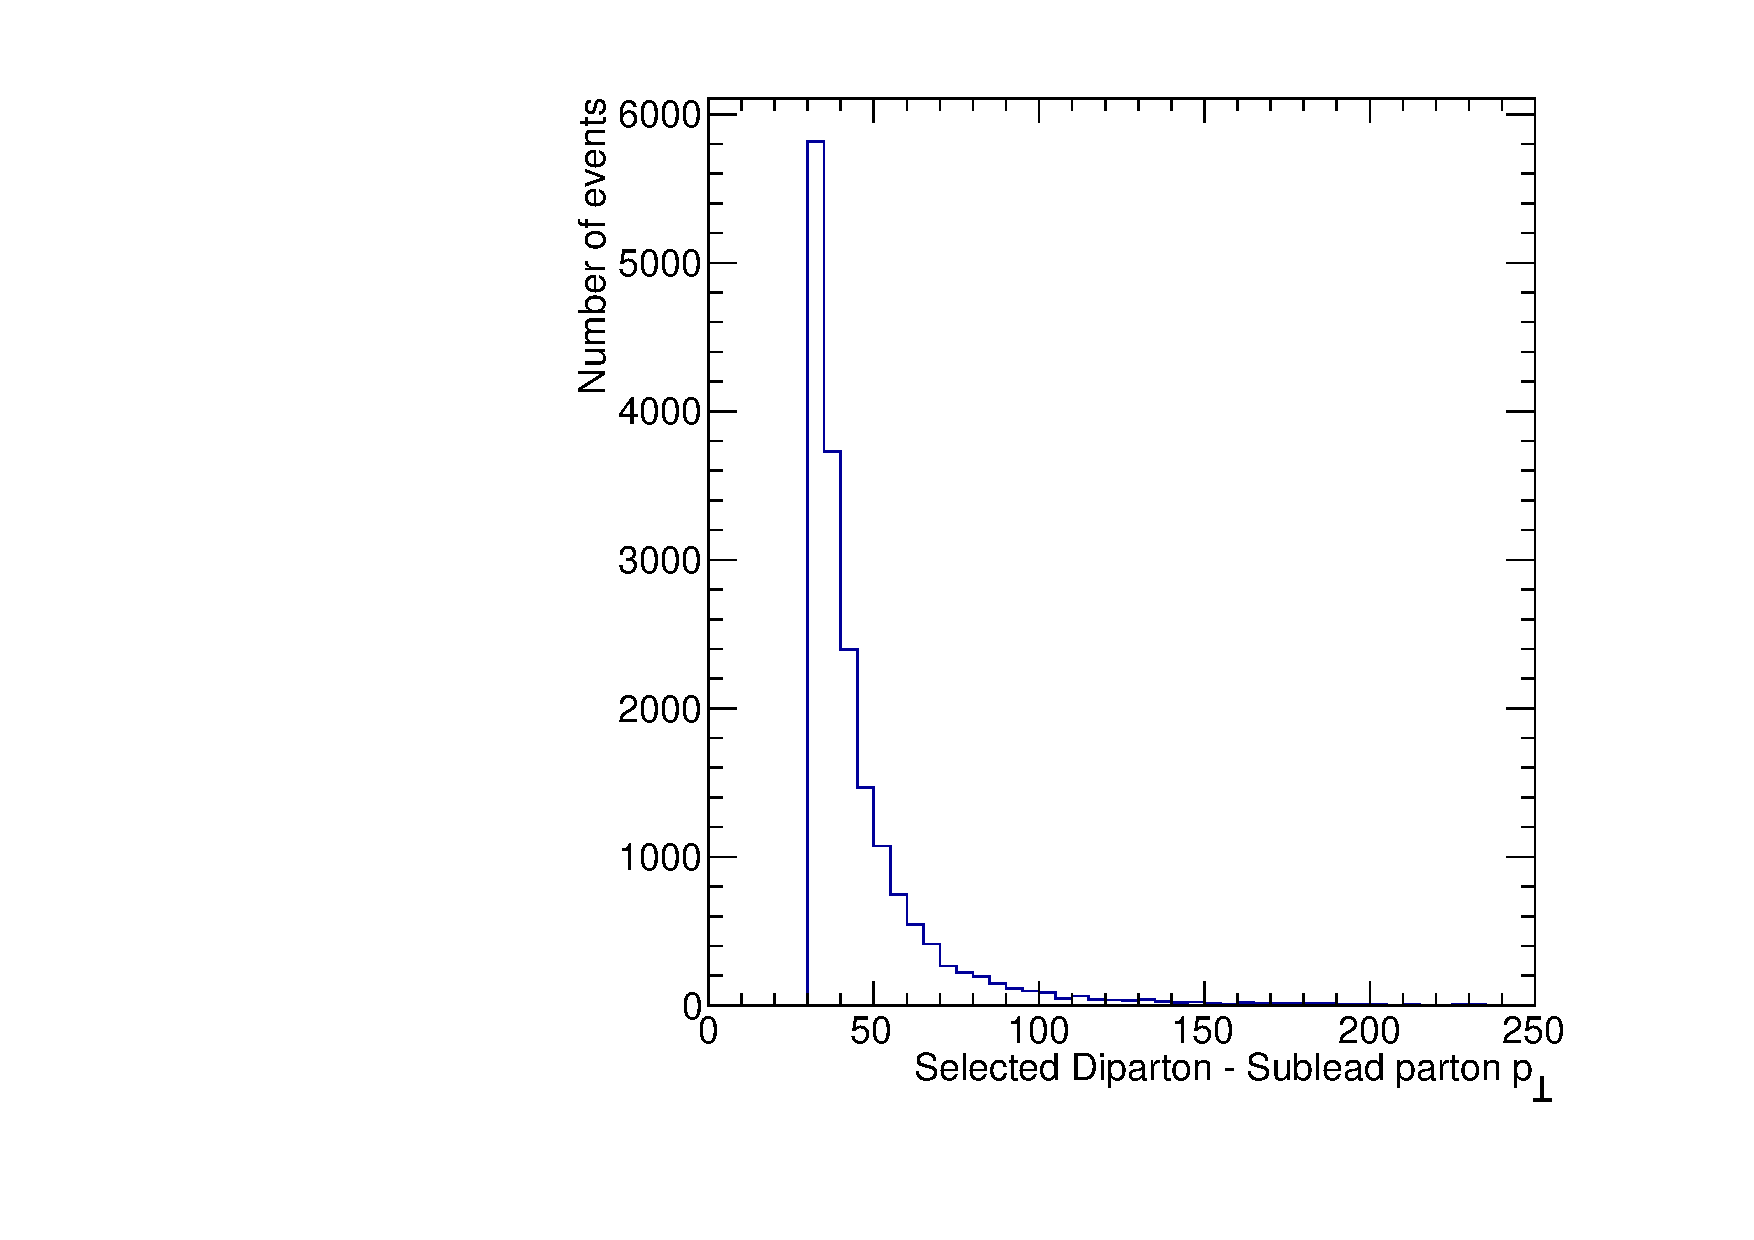
\includegraphics[width=0.45\linewidth]{Chapter07/QCDVBFSamples/Gridpack/Images/SelDiParton_Parton2_Pt.pdf}}\\
\caption[TODO]{TODO}
\label{FIGURE:TODO}
\end{figure}

\begin{figure}[htp]%
\centering
\subfloat[][]{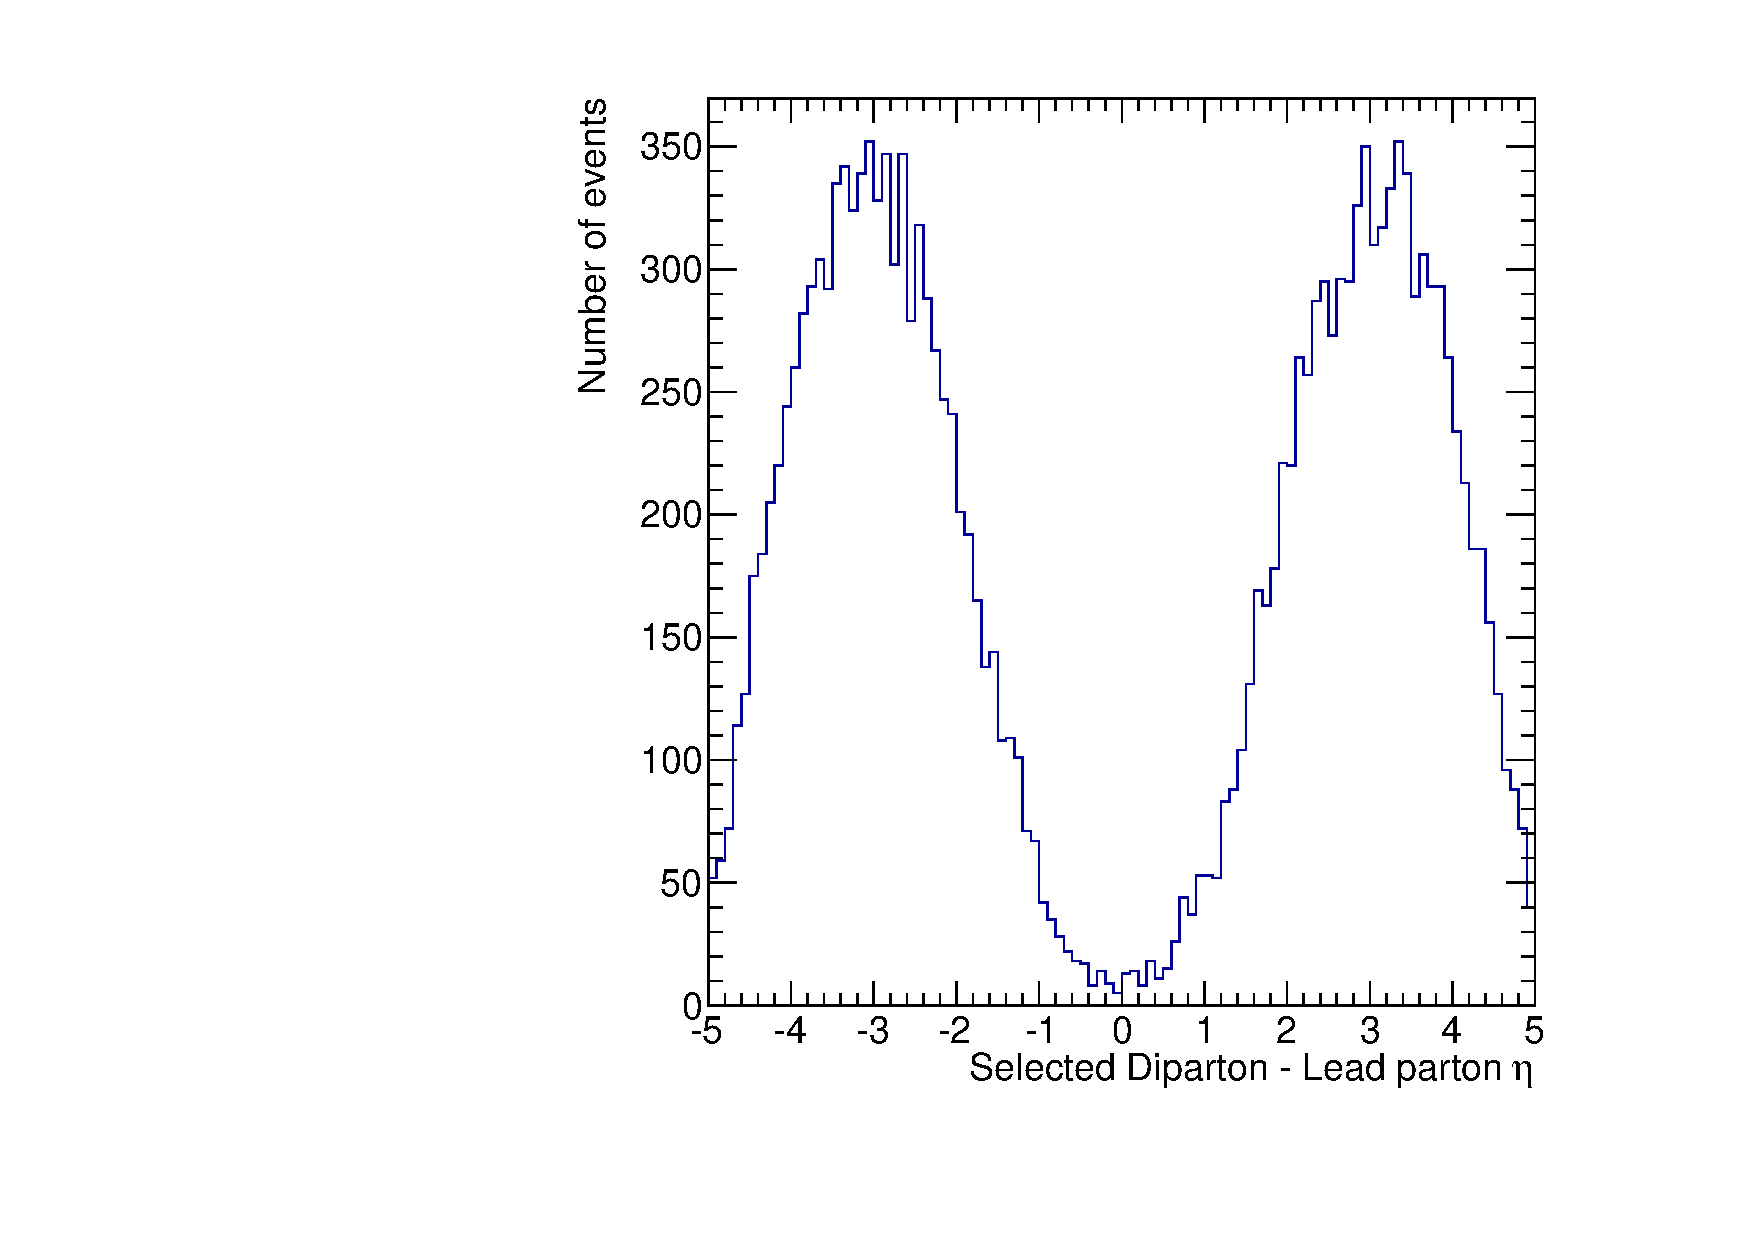
\includegraphics[width=0.45\linewidth]{Chapter07/QCDVBFSamples/Gridpack/Images/SelDiParton_Parton1_Eta.pdf}}\qquad
\subfloat[][]{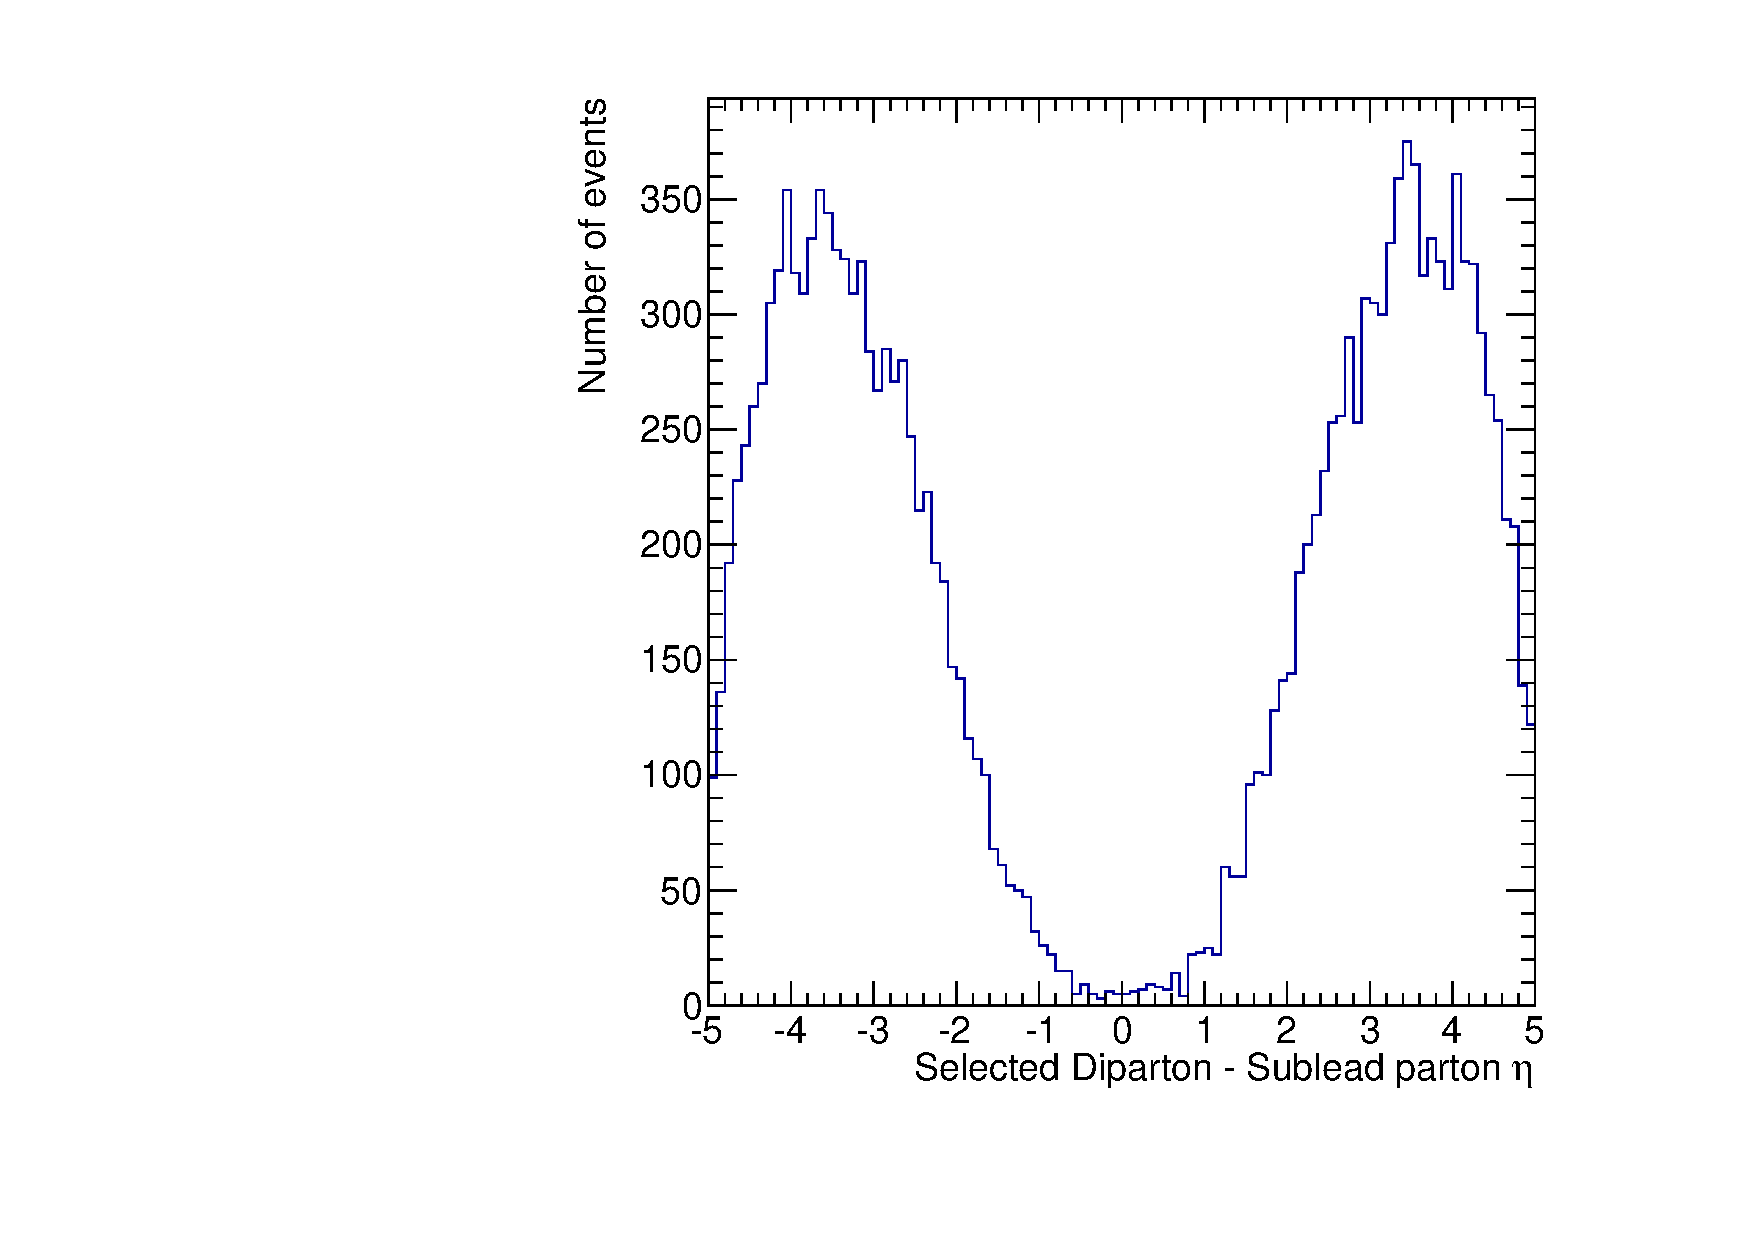
\includegraphics[width=0.45\linewidth]{Chapter07/QCDVBFSamples/Gridpack/Images/SelDiParton_Parton2_Eta.pdf}}\\
\caption[TODO]{TODO}
\label{FIGURE:TODO}
\end{figure}

\begin{figure}[htp]%
\centering
\subfloat[][]{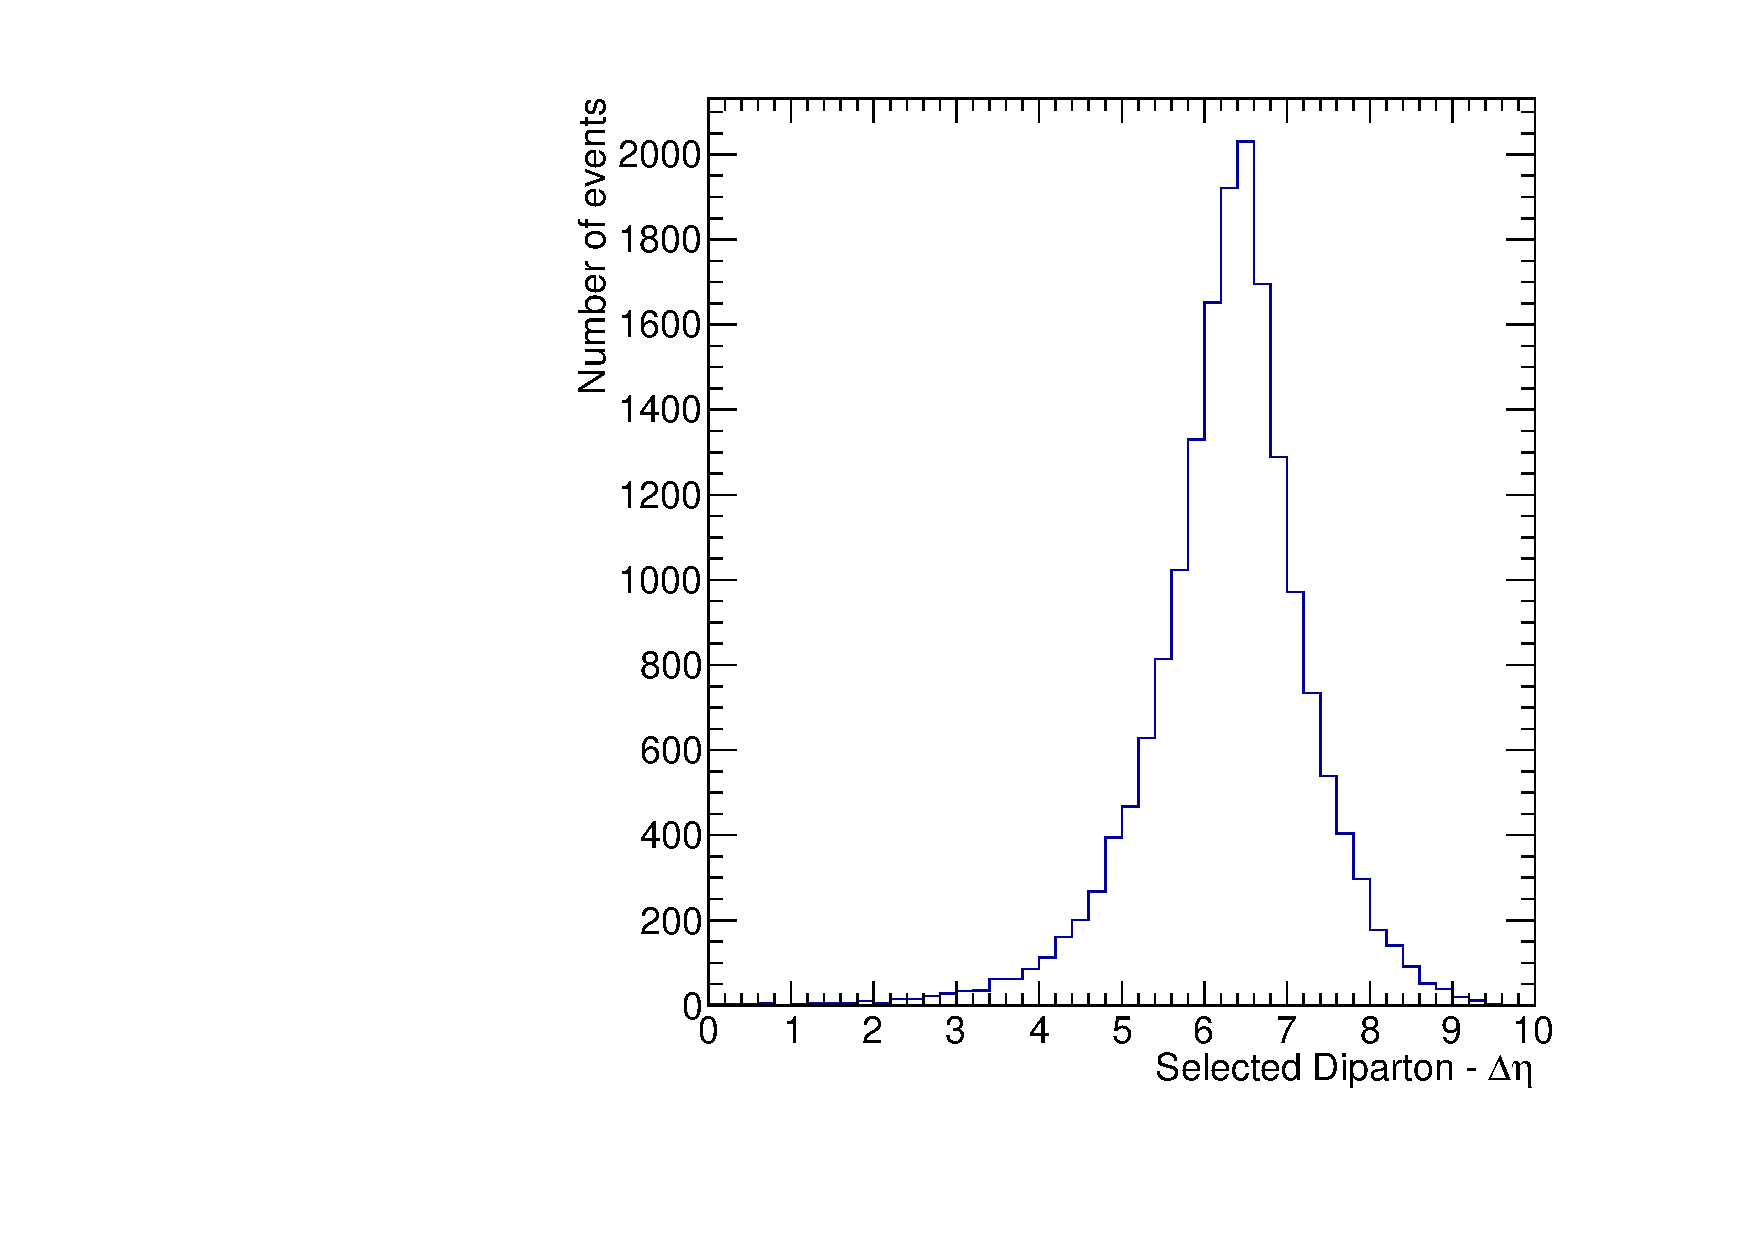
\includegraphics[width=0.45\linewidth]{Chapter07/QCDVBFSamples/Gridpack/Images/SelDiParton_DEta.pdf}}\qquad
\subfloat[][]{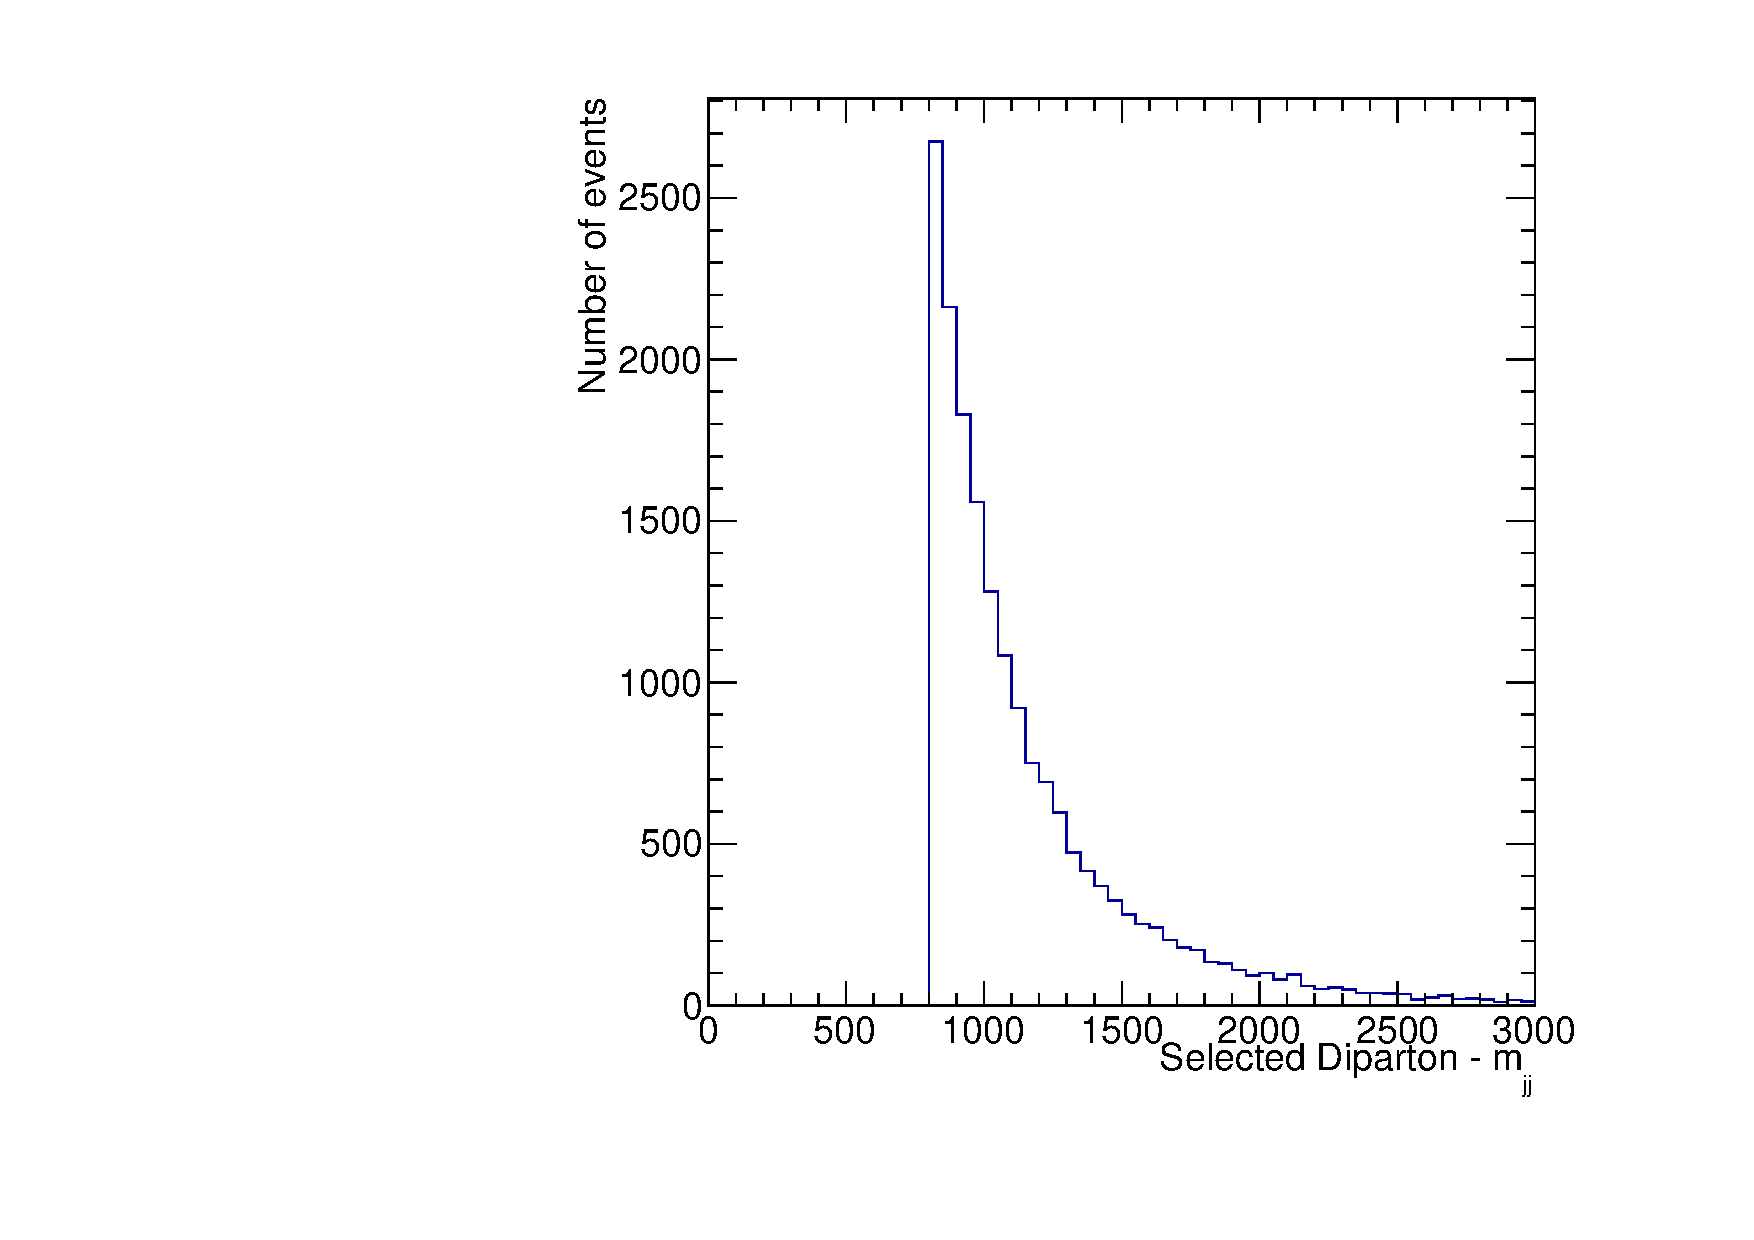
\includegraphics[width=0.45\linewidth]{Chapter07/QCDVBFSamples/Gridpack/Images/SelDiParton_Mjj.pdf}}\\
\caption[TODO]{TODO}
\label{FIGURE:TODO}
\end{figure}

\begin{figure}[htp]%
\centering
\subfloat[][]{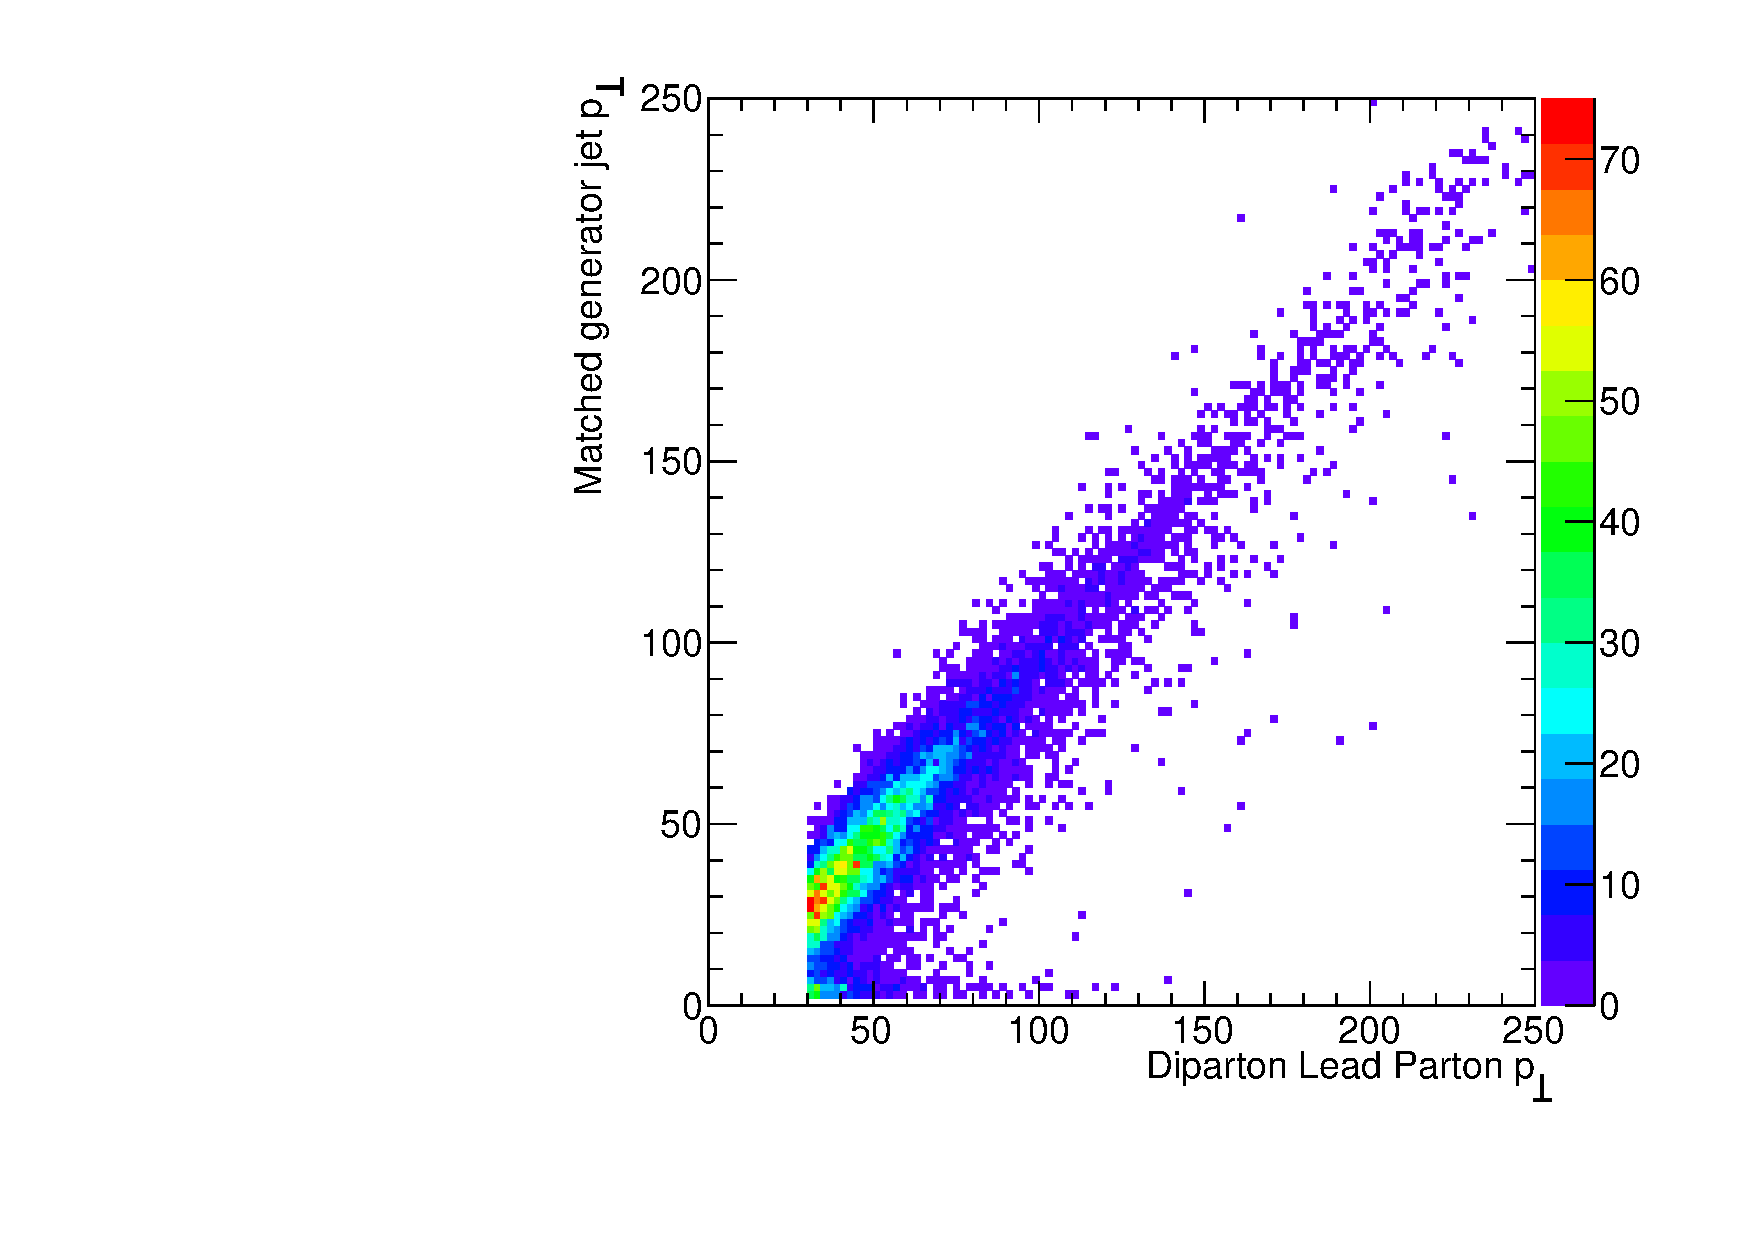
\includegraphics[width=0.45\linewidth]{Chapter07/QCDVBFSamples/Gridpack/Images/SelDiParton_MatchedGenJet_Parton1_Pt.pdf}}\qquad
\subfloat[][]{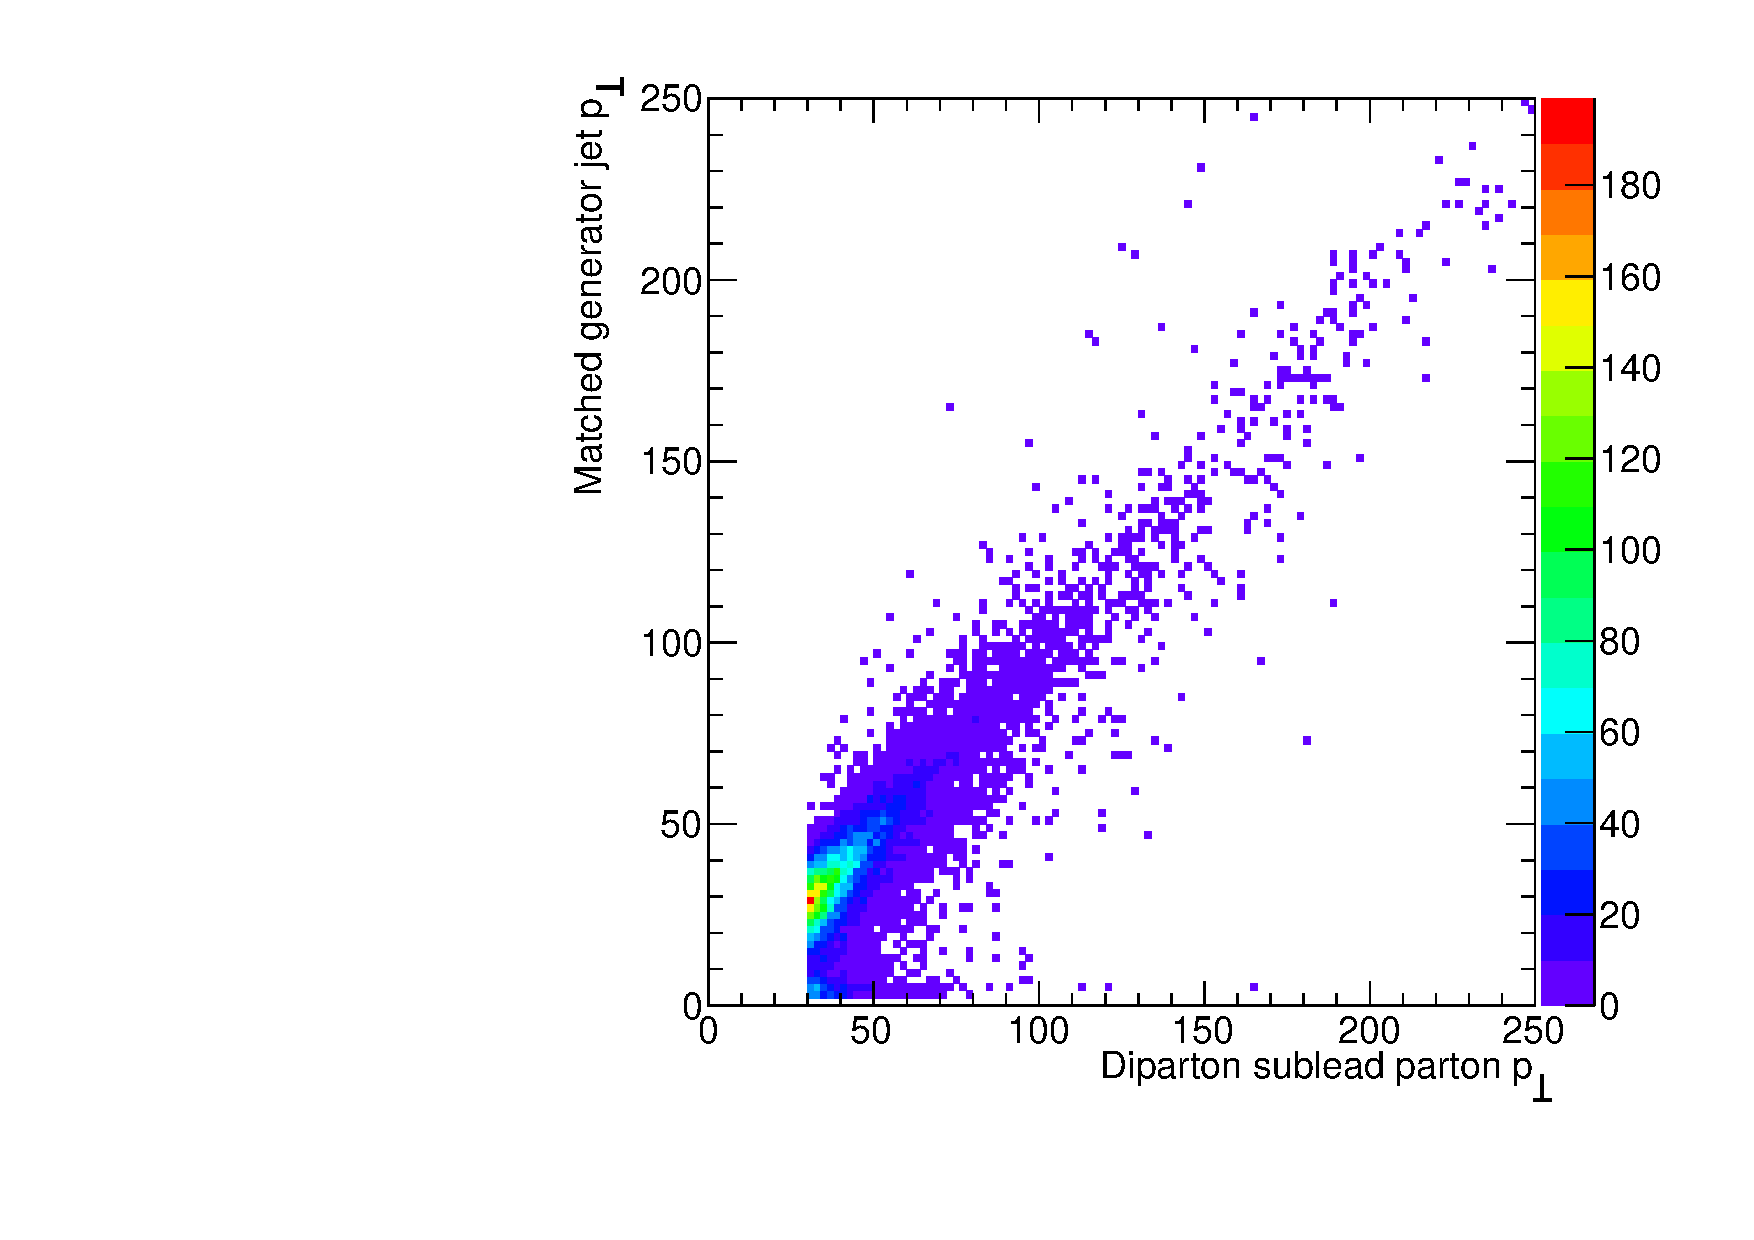
\includegraphics[width=0.45\linewidth]{Chapter07/QCDVBFSamples/Gridpack/Images/SelDiParton_MatchedGenJet_Parton2_Pt.pdf}}\\
\caption[TODO]{TODO}
\label{FIGURE:TODO}
\end{figure}

\begin{figure}[htp]%
\centering
\subfloat[][]{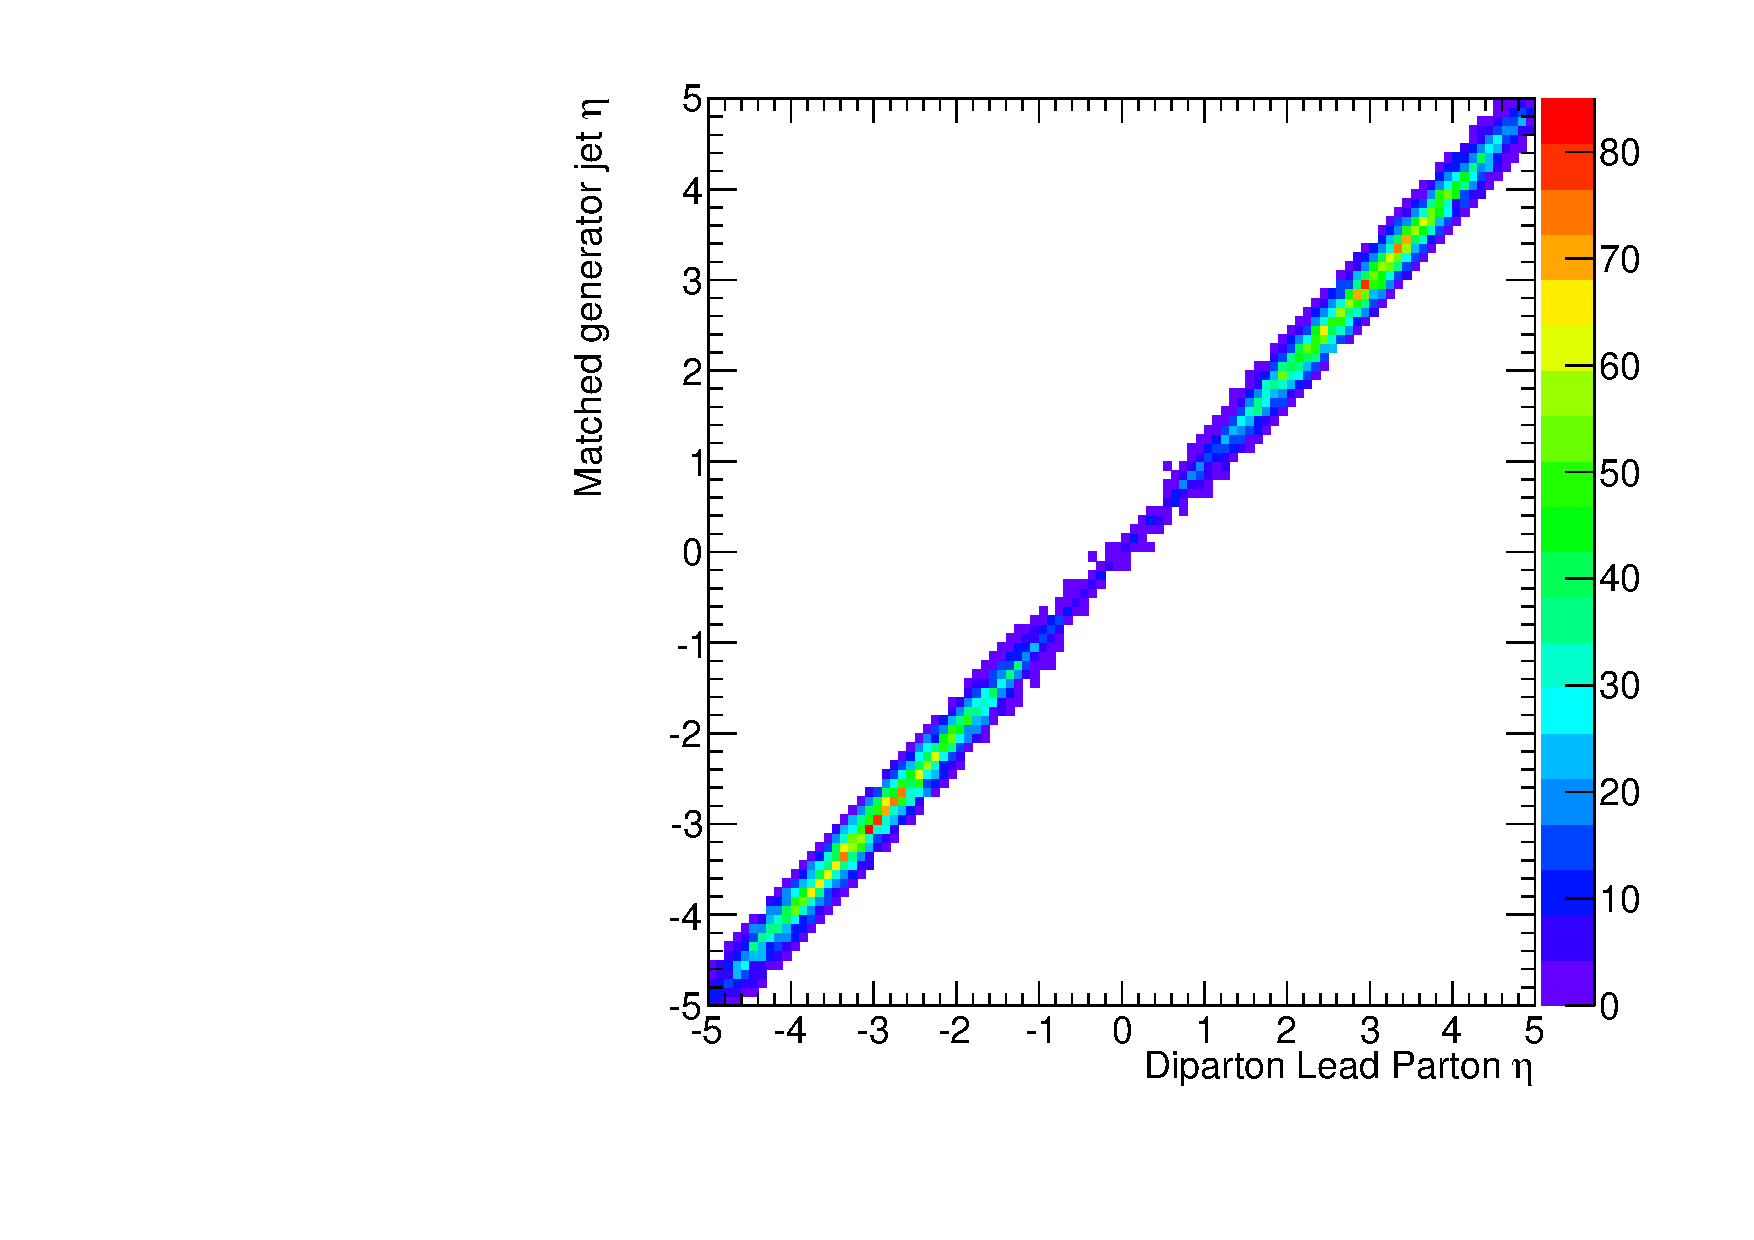
\includegraphics[width=0.45\linewidth]{Chapter07/QCDVBFSamples/Gridpack/Images/SelDiParton_MatchedGenJet_Parton1_Eta.pdf}}\qquad
\subfloat[][]{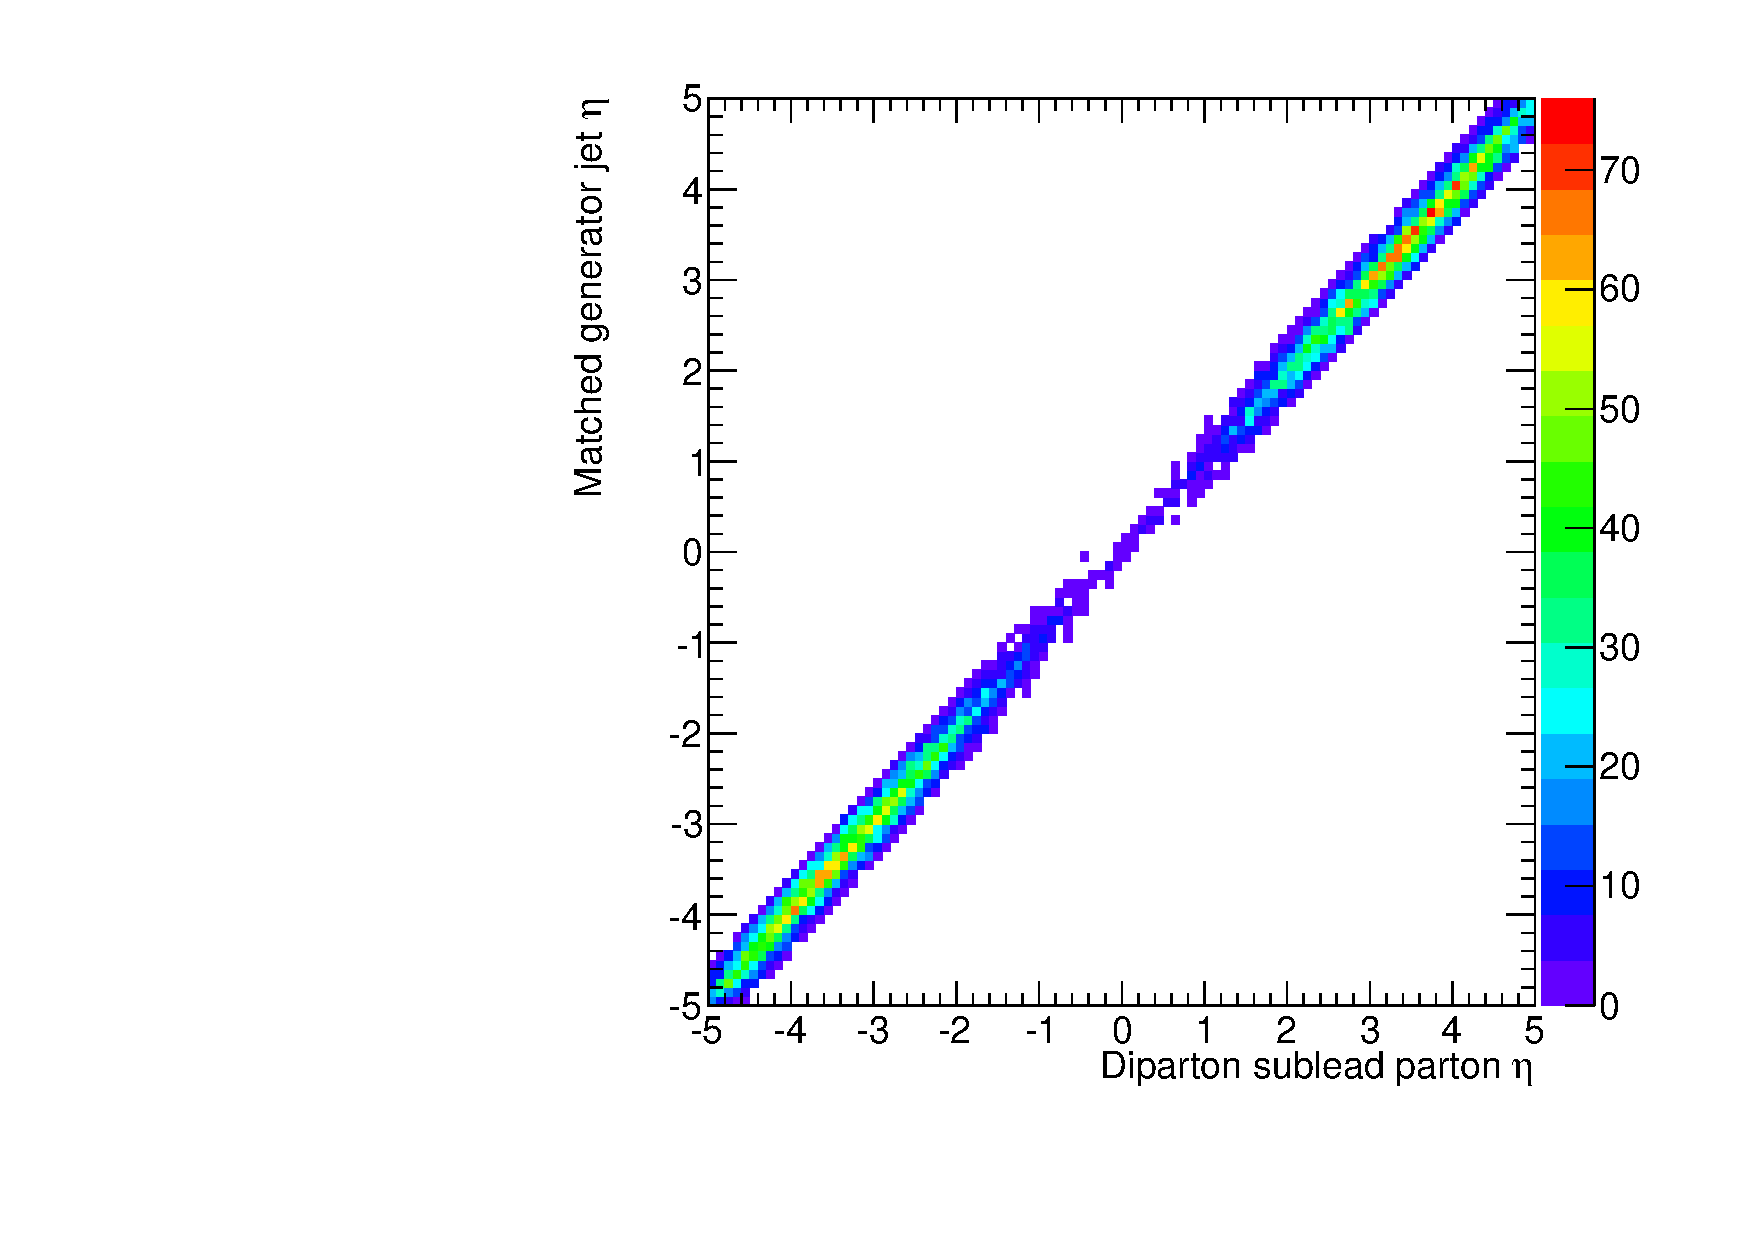
\includegraphics[width=0.45\linewidth]{Chapter07/QCDVBFSamples/Gridpack/Images/SelDiParton_MatchedGenJet_Parton2_Eta.pdf}}\\
\caption[TODO]{TODO}
\label{FIGURE:TODO}
\end{figure}

\begin{figure}[htp]%
\centering
\subfloat[][]{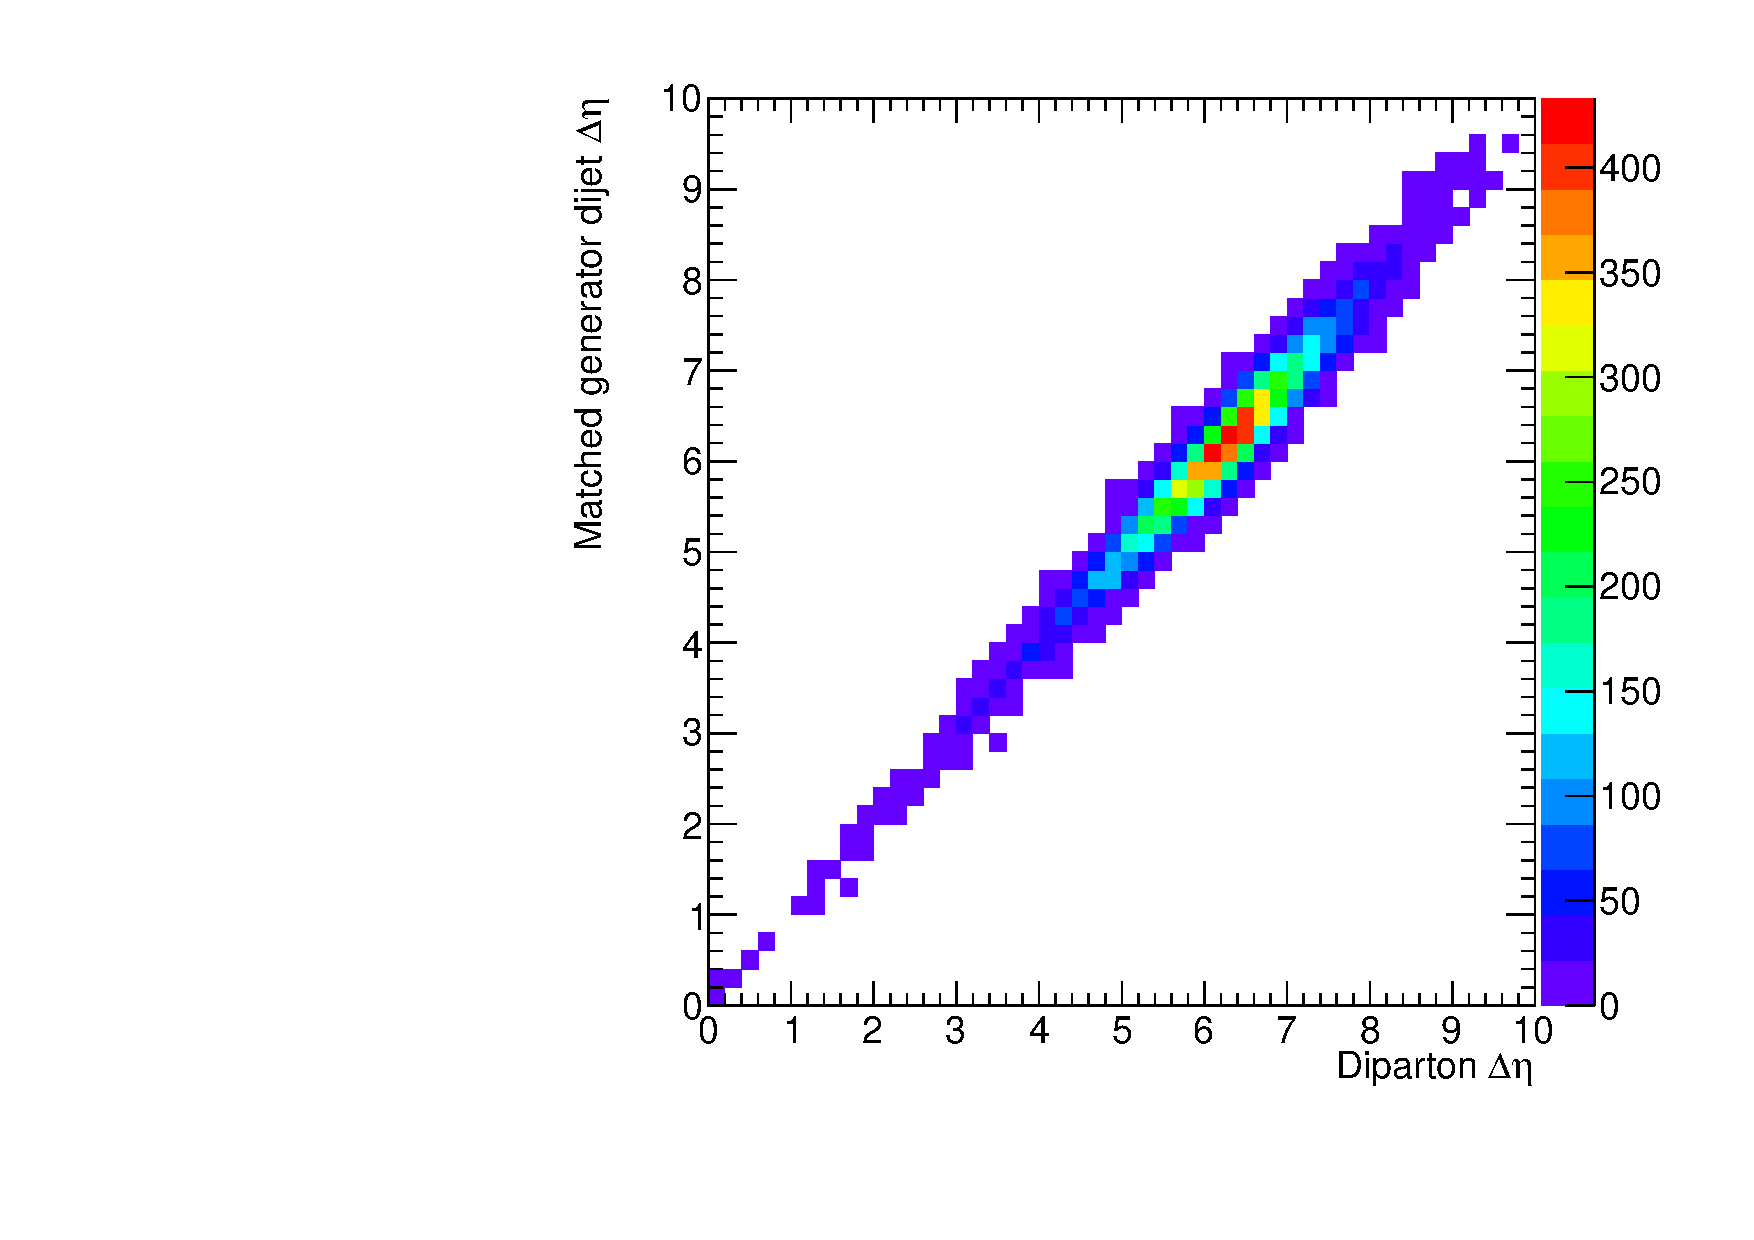
\includegraphics[width=0.45\linewidth]{Chapter07/QCDVBFSamples/Gridpack/Images/SelDiParton_MatchedGenJet_DEta.pdf}}\qquad
\subfloat[][]{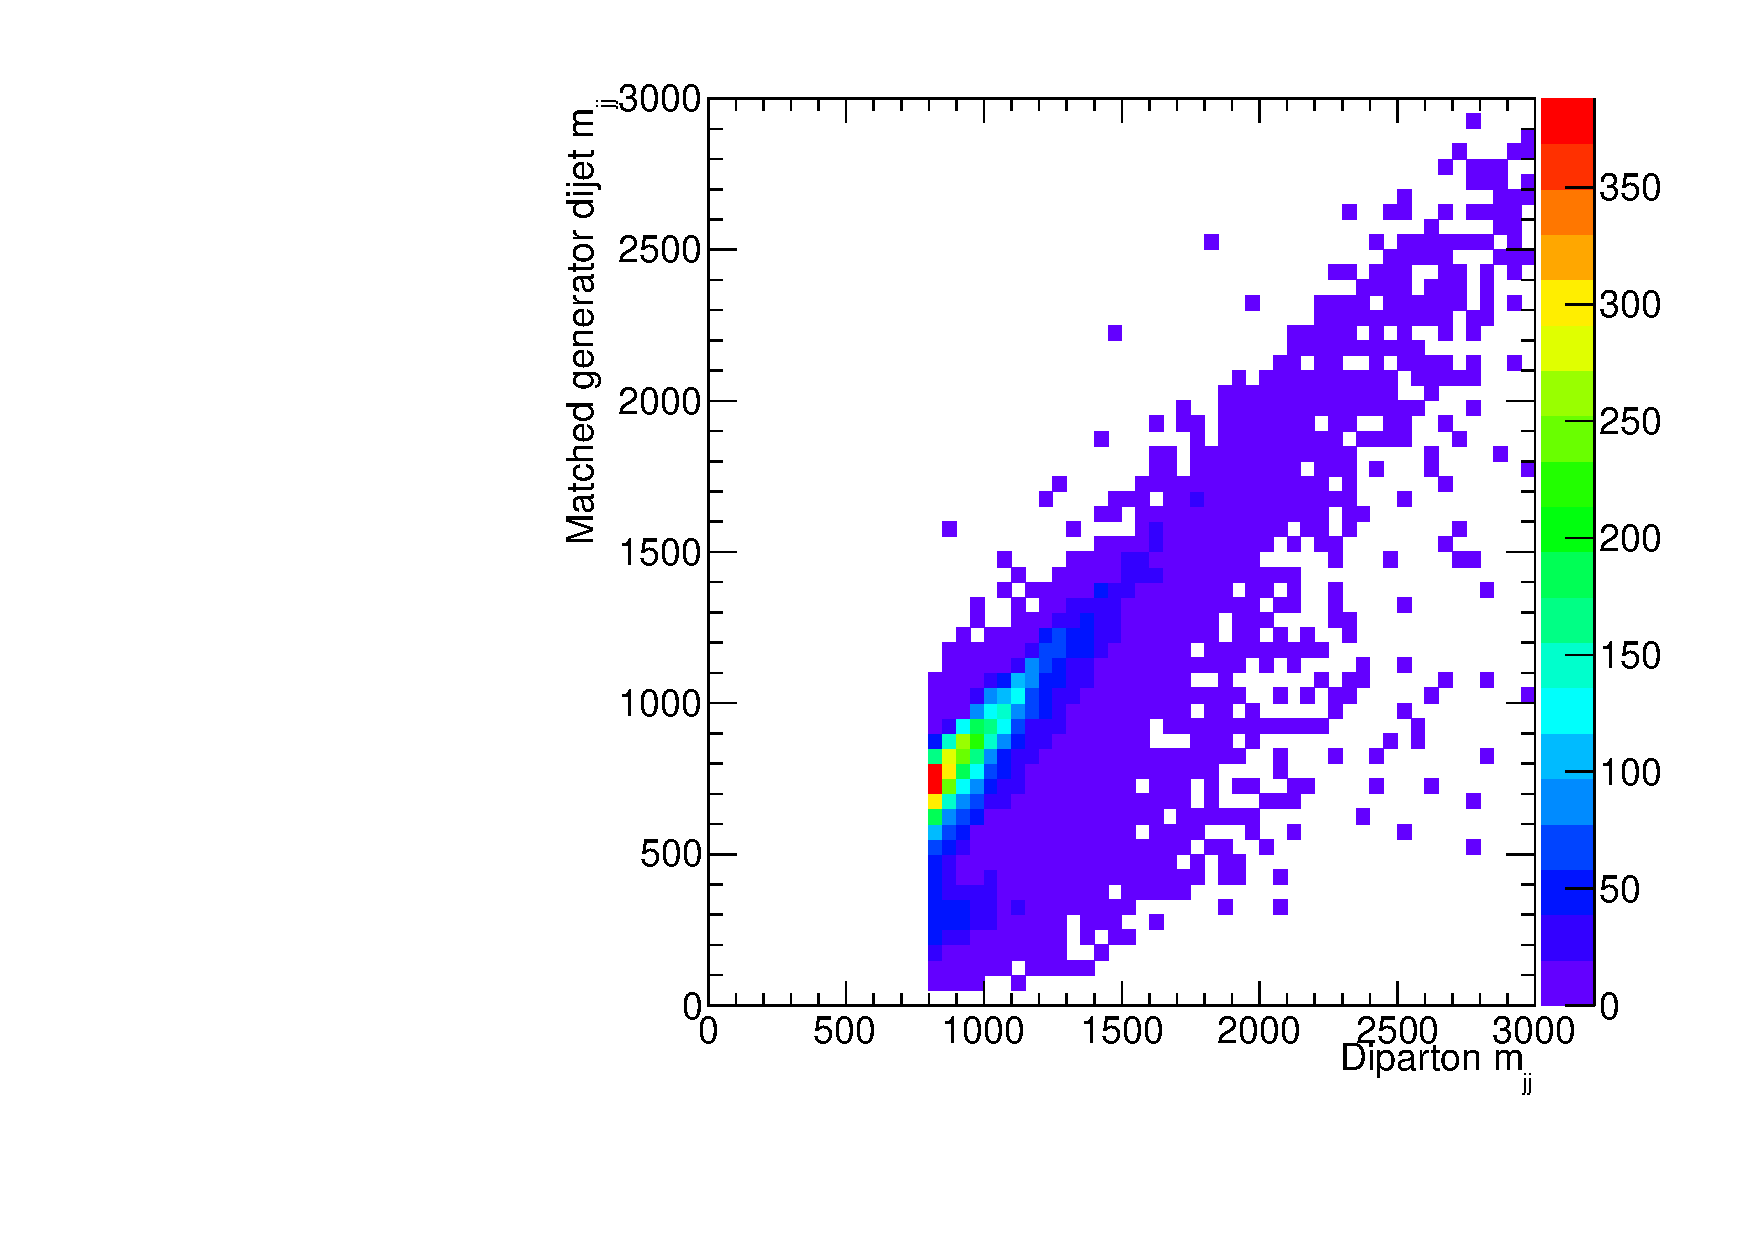
\includegraphics[width=0.45\linewidth]{Chapter07/QCDVBFSamples/Gridpack/Images/SelDiParton_MatchedGenJet_Mjj.pdf}}\\
\caption[TODO]{TODO}
\label{FIGURE:TODO}
\end{figure}

\subsubsection{Migration study}

A second gridpack was setup with lower parton cuts in order to study event migrations between the thresholds of the parton filter and the generator jets filter.

Single variable migration (Lead $p_T$)
\begin{equation}
\frac{p_{\perp}^{Parton}<30 \text{ AND } p_{\perp}^{GenJet} \geq 40}{p_{\perp}^{GenJet} \geq 40}=0.27\% \pm 0.04\%
\end{equation}

Single variable migration (Sub-lead $p_T$)
\begin{equation}
\frac{p_{\perp}^{Parton}<30 \text{ AND } p_{\perp}^{GenJet} \geq 40}{p_{\perp}^{GenJet} \geq 40}=0.56\% \pm 0.08\%
\end{equation}

Single variable migration ($m_{jj}$)
\begin{equation}
\frac{m_{jj}^{Parton}<800 \text{ AND } m_{jj}^{GenJet} \geq 1000}{m_{jj}^{GenJet} \geq 800}=0.13\% \pm 0.04\%
\end{equation}

Double variable migration
\begin{equation}
\frac{(p_{\perp}^{GenJet}>40 \text{ AND } m_{jj}^{GenJet}>1000) \text{ AND } (p_{\perp}^{Parton}<30 \text{ OR } m_{jj}^{Parton}<800)}{p_{\perp}^{GenJet}>40 \text{ AND } m_{jj}^{GenJet}>1000} = 0.23\% \pm 0.13\%
\end{equation}

\subsubsection{Generator level cuts}

% girdpack2
% \begin{itemize}
%   \item Starting 30699
%   \item OppSide_Dijet40_Eta4p8_DEta3p0_Mjj1000          - 4159 (from analysis code)
%   \item OppSide_Dijet40_Eta4p8_DEta3p0_Mjj1000          - 4159 (from filter code)
%   \item OppSide_Dijet40_Eta4p8_DEta3p0_Mjj1000_DPhi2.15 - 867 (from analysis code)
%   \item OppSide_Dijet40_Eta4p8_DEta3p0_Mjj1000_DPhi2.15 - 867 (from filter code)
%   \item Events above cuts 867 (eff 0.028241962 +/- 0.00095914732)
%   \item OppSide_Dijet40_Eta4p8_DEta3p0_Mjj1000_BiggerDPhi2.15 - 3448 (from filter code)
%   \item Events above cuts 3448 (eff 0.11231636 +/- 0.0019127552)
%   \item Dijet40_Eta4p8_DEta3p0_Mjj1000_DPhi2.15       - 867  (from filter code)
%   \item Dijet40_Eta4p8_DEta3p0_Mjj1000_BiggerDPhi2.15 - 3452 (from filter code)
% \end{itemize}
 
\begin{table}[!htp]
\centering
\begin{tabular}{|c||c|c|c|}
\hline
           & \multicolumn{3}{c|}{$\Delta\phi$ cut} \\
\hline
$N_{Jets}$ & no cut        & $<2.15$        & $\gtrsim 2.15$ \\
\hline\hline
 2         & 63.83 \pm 0.59 & 15.80 \pm 0.63 & 73.38 \pm 0.70 \\
 3         & 23.53 \pm 0.36 & 50.21 \pm 1.13 & 17.59 \pm 0.34 \\
 4         &  9.43 \pm 0.23 & 24.34 \pm 0.78 &  6.70 \pm 0.21 \\
 5         &  2.42 \pm 0.11 &  7.14 \pm 0.42 &  1.70 \pm 0.11 \\
+6         &  0.79 \pm 0.07 &  2.50 \pm 0.25 &  0.63 \pm 0.06 \\
\hline
\end{tabular}
\caption[Table showing the percentage of events for a given multiplicity of generator anti-$k_T$ jets with $R=0.4$ passing cuts $p_T>40\,\GeV$ and $|\eta|<4.8$. Only events with at least one such dijet with $\Delta\eta<3.0$ and $m_{jj}<1000\,\GeV$ are considered and results are presented according to a possible additional dijet $\Delta\phi$ cut.]
{Table showing the percentage of events for a given multiplicity of generator anti-$k_T$ jets with $R=0.4$ passing cuts $p_T>40\,\GeV$ and $|\eta|<4.8$. Only events with at least one such dijet with $\Delta\eta<3.0$ and $m_{jj}<1000\,\GeV$ are considered and results are presented according to a possible additional dijet $\Delta\phi$ cut.}
\label{TABLE:RunIIPreparation_PassFilterNJetsDphi}
\end{table}

% Information extracted to do this table:
%#######################################################
% Printing cuts: Pt40_Eta4p8_DEta3p0_Mjj1000
%#######################################################
% => Number Jets Passing pT and Eta cuts multiplicity (at least one combination passes all cuts):
% N_Jets= 0 entries=         0 fraction=0.000000 +/- 0.000000
% N_Jets= 1 entries=         0 fraction=0.000000 +/- 0.000000
% N_Jets= 2 entries=     11757 fraction=0.638274 +/- 0.005887
% N_Jets= 3 entries=      4335 fraction=0.235342 +/- 0.003574
% N_Jets= 4 entries=      1737 fraction=0.094300 +/- 0.002263
% N_Jets= 5 entries=       446 fraction=0.024213 +/- 0.001147
% N_Jets= 6 entries=       117 fraction=0.006352 +/- 0.000587
% N_Jets= 7 entries=        22 fraction=0.001194 +/- 0.000255
% N_Jets= 8 entries=         4 fraction=0.000217 +/- 0.000109
% N_Jets= 9 entries=         2 fraction=0.000109 +/- 0.000077
% N_Jets=10 entries=         0 fraction=0.000000 +/- 0.000000
%####################################################### 
% N_Jets=+6 entries=       145 fraction=0.007872 +/- 0.000654
%#######################################################
%
%
%######################################################
%Printing cuts: Pt40_Eta4p8_DEta3p0_Dphi2p15_Mjj1000
%######################################################
% => Number Jets Passing pT and Eta cuts multiplicity (at least one combination passes all cuts):
% N_Jets= 0 entries=         0 fraction=0.000000 +/- 0.000000
% N_Jets= 1 entries=         0 fraction=0.000000 +/- 0.000000
% N_Jets= 2 entries=       626 fraction=0.158041 +/- 0.006317
% N_Jets= 3 entries=      1989 fraction=0.502146 +/- 0.011259
% N_Jets= 4 entries=       964 fraction=0.243373 +/- 0.007839
% N_Jets= 5 entries=       283 fraction=0.071447 +/- 0.004247
% N_Jets= 6 entries=        81 fraction=0.020449 +/- 0.002272
% N_Jets= 7 entries=        15 fraction=0.003787 +/- 0.000978
% N_Jets= 8 entries=         2 fraction=0.000505 +/- 0.000357
% N_Jets= 9 entries=         1 fraction=0.000252 +/- 0.000252
% N_Jets=10 entries=         0 fraction=0.000000 +/- 0.000000
%####################################################### 
% N_Jets=+6 entries=        99 fraction=0.024994 +/- 0.002512
%####################################################### 
%
%
%#######################################################
%Printing cuts: Pt40_Eta4p8_DEta3p0_MinDphi2p15_Mjj1000
%####################################################### 
% => Number Jets Passing pT and Eta cuts multiplicity (at least one combination passes all cuts):
% N_Jets= 0 entries=         0 fraction=0.000000 +/- 0.000000
% N_Jets= 1 entries=         0 fraction=0.000000 +/- 0.000000
% N_Jets= 2 entries=     11131 fraction=0.733799 +/- 0.006955
% N_Jets= 3 entries=      2668 fraction=0.175885 +/- 0.003405
% N_Jets= 4 entries=      1017 fraction=0.067045 +/- 0.002102
% N_Jets= 5 entries=       258 fraction=0.017008 +/- 0.001059
% N_Jets= 6 entries=        75 fraction=0.004944 +/- 0.000571
% N_Jets= 7 entries=        15 fraction=0.000989 +/- 0.000255
% N_Jets= 8 entries=         3 fraction=0.000198 +/- 0.000114
% N_Jets= 9 entries=         2 fraction=0.000132 +/- 0.000093
% N_Jets=10 entries=         0 fraction=0.000000 +/- 0.000000
%#######################################################
% N_Jets=+6 entries=        95 fraction=0.006263 +/- 0.000643
%#######################################################


\begin{table}[!htp]
\centering
\begin{tabular}{|c|c|c|c|}
\hline
           & \multicolumn{3}{c|}{$\Delta\phi$ cut} \\
\hline
$N_{Jets}$ & no cut        & $<2.15$        & $\gtrsim 2.15$ \\
\hline\hline
 1         & 93.53 \pm 0.71 & 94.29 \pm 1.54 & 97.51 \pm 0.80 \\
 2         &  5.84 \pm 0.18 &  5.35 \pm 0.37 &  2.39 \pm 0.13 \\
 3         &  0.44 \pm 0.05 &  0.30 \pm 0.09 &  0.07 \pm 0.02 \\
+4         &  0.19 \pm 0.03 &  0.05 \pm 0.04 &  0.03 \pm 0.01 \\
\hline
\end{tabular}
\caption{Table showing the percentage of generator AK4 dijets passing cuts $p_T^{jet}>40\,\GeV$, $|\eta|^{jet}<4.8$, $\Delta\eta<3.0$ and $m_{jj}<1000\,\GeV$ and according to an additional dijet $\Delta\phi$ cut.}
\end{table}

% #######################################################
% Printing cuts: Pt40_Eta4p8_DEta3p0_Mjj1000
% #######################################################
% => Dijets passing all cuts multiplicity:
% N_Dijets= 0 entries=         0 fraction=0.000000 +/- 0.000000
% N_Dijets= 1 entries=     17228 fraction=0.935288 +/- 0.007126
% N_Dijets= 2 entries=      1076 fraction=0.058415 +/- 0.001781
% N_Dijets= 3 entries=        81 fraction=0.004397 +/- 0.000489
% N_Dijets= 4 entries=        31 fraction=0.001683 +/- 0.000302
% N_Dijets= 5 entries=         2 fraction=0.000109 +/- 0.000077
% N_Dijets= 6 entries=         2 fraction=0.000109 +/- 0.000077
% N_Dijets= 7 entries=         0 fraction=0.000000 +/- 0.000000
% N_Dijets= 8 entries=         0 fraction=0.000000 +/- 0.000000
% N_Dijets= 9 entries=         0 fraction=0.000000 +/- 0.000000
% N_Dijets=10 entries=         0 fraction=0.000000 +/- 0.000000
% ####################################################### 
% N_Dijets=+4 entries=        35 fraction=0.001900 +/- 0.000321
% #######################################################
%
% 
% #######################################################
% Printing cuts: Pt40_Eta4p8_DEta3p0_Dphi2p15_Mjj1000
% #######################################################
% => Dijets passing all cuts multiplicity:
% N_Dijets= 0 entries=         0 fraction=0.000000 +/- 0.000000
% N_Dijets= 1 entries=      3735 fraction=0.942944 +/- 0.015429
% N_Dijets= 2 entries=       212 fraction=0.053522 +/- 0.003676
% N_Dijets= 3 entries=        12 fraction=0.003030 +/- 0.000875
% N_Dijets= 4 entries=         2 fraction=0.000505 +/- 0.000357
% N_Dijets= 5 entries=         0 fraction=0.000000 +/- 0.000000
% N_Dijets= 6 entries=         0 fraction=0.000000 +/- 0.000000
% N_Dijets= 7 entries=         0 fraction=0.000000 +/- 0.000000
% N_Dijets= 8 entries=         0 fraction=0.000000 +/- 0.000000
% N_Dijets= 9 entries=         0 fraction=0.000000 +/- 0.000000
% N_Dijets=10 entries=         0 fraction=0.000000 +/- 0.000000
% ####################################################### 
%
% #######################################################
% 
% 
% #######################################################
% Printing cuts: Pt40_Eta4p8_DEta3p0_MinDphi2p15_Mjj1000
% #######################################################
% => Dijets passing all cuts multiplicity:
% N_Dijets= 0 entries=         0 fraction=0.000000 +/- 0.000000
% N_Dijets= 1 entries=     14791 fraction=0.975081 +/- 0.008018
% N_Dijets= 2 entries=       363 fraction=0.023930 +/- 0.001256
% N_Dijets= 3 entries=        11 fraction=0.000725 +/- 0.000219
% N_Dijets= 4 entries=         4 fraction=0.000264 +/- 0.000132
% N_Dijets= 5 entries=         0 fraction=0.000000 +/- 0.000000
% N_Dijets= 6 entries=         0 fraction=0.000000 +/- 0.000000
% N_Dijets= 7 entries=         0 fraction=0.000000 +/- 0.000000
% N_Dijets= 8 entries=         0 fraction=0.000000 +/- 0.000000
% N_Dijets= 9 entries=         0 fraction=0.000000 +/- 0.000000
% N_Dijets=10 entries=         0 fraction=0.000000 +/- 0.000000
% ####################################################### 
%
% #######################################################

